\documentclass{article}
\usepackage[utf8]{inputenc}
\usepackage[italian]{babel}
\usepackage{amsmath}
\usepackage{amssymb}
\usepackage{siunitx}
\usepackage{tabularray}
\usepackage{graphicx}
\usepackage{float}
\usepackage{xfrac}
\usepackage[justification=centering]{caption}    % for \caption*{}
\usepackage[bottom]{footmisc}
\usepackage[labelformat=simple, justification=centering]{subfig}
\renewcommand{\thesubfigure}{}
\newcommand*{\diam}{\varnothing}
\newcommand*{\best}[1]{{#1}_\text{best}}
\newcommand*{\bestp}[1]{{\left(#1\right)}_\text{best}}
\newcommand*{\pbest}[1]{\left({#1}_\text{best}\right)}
\newcommand*{\pbestp}[1]{\left({\left(#1\right)}_\text{best}\right)}
\newcommand*{\errrel}[1]{\frac{\delta #1}{{#1}_\text{best}}}
%% <custom footnotes/>
%\newcounter{savefootnote}
%\newcounter{symfootnote}
%\newcommand{\symfootnote}[1]{%
%   \setcounter{savefootnote}{\value{footnote}}%
%   \setcounter{footnote}{\value{symfootnote}}%
%   \ifnum\value{footnote}>8\setcounter{footnote}{0}\fi%
%   \let\oldthefootnote=\thefootnote%
%   \renewcommand{\thefootnote}{\fnsymbol{footnote}}%
%   \footnote{#1}%
%   \let\thefootnote=\oldthefootnote%
%   \setcounter{symfootnote}{\value{footnote}}%
%   \setcounter{footnote}{\value{savefootnote}}%
%}
%% </custom footnotes>
\title{
  Laboratorio di Fisica 1\\
  R8: Taratura di una termocoppia
}
\author{Gruppo 15: Bergamaschi Riccardo, Moglia Simone, Graiani Elia}
\date{30/04/2024 – 07/05/2024}
\makeindex
\begin{document}

\maketitle

\begin{abstract}
  Il gruppo di lavoro ha determinato la curva di calibrazione di una
  termocoppia sfruttando punti fissi, ovvero temperature note,
  di svariate sostanze chimiche.
\end{abstract}

\setcounter{section}{-1}  % Count sections starting from 0
\section{Materiali e strumenti di misura utilizzati}
\begin{center}
  \begin{tblr}{
    width=\textwidth,
    colspec={ X[2,m,j]X[m,c]X[m,c]X[m,c] },
    vlines,
  }
    \hline
    \textbf{Strumento di misura} & \textbf{Soglia} & \textbf{Portata} & \textbf{Sensibilità} \\
    \hline
    Termocoppia (tipo K) & \qty{-6.03}{mV} & \qty{50.64}{mV} & \qty{0.01}{mV} \\
    \hline[dashed]
    Cronometro & \qty{0.01}{s} & N./A. & \qty{0.01}{s} \\
    \hline[dashed]
    Termometro ambientale & \qty{-10.0}{\degree C}? & \qty{50.64}{\degree C}? & \qty{0.5}{\degree C} \\
    \hline
  \end{tblr}
  \begin{tblr}{
    width=\textwidth,
    colspec={ X[2,m,j]X[3,m,j] },
    vlines,
  }
    \hline
    \textbf{Altro} & \textbf{Descrizione/Note} \\
    \hline
    Campioni di sostanze chimiche & {
      Azoto liquido, acqua distillata,
      etanolo, gallio, e indio.
    } \\
    \hline[dashed]
    Amplificatore di voltaggio & {
      Amplifica di un fattore 100 il voltaggio rilevato dalla
      termocoppia, rendendo possibile l'acquisizione dati.
    } \\
    \hline[dashed]
    Fornelletto e pentolino & Per scaldare i campioni. \\
    \hline[dashed]
    Cacciavite & Utilizzato per collegare la termocoppia all'interfaccia. \\
    \hline[dashed]
    { Guanto da forno, pinzette, presine e contenitori isolanti } & {
      Per maneggiare i campioni in sicurezza.
    } \\
    \hline
  \end{tblr}
\end{center}

\pagebreak
\section{Esperienza e procedimento di misura}

\begin{enumerate}
  \item
    Posizioniamo una giunzione della termocoppia (che d'ora in poi indicheremo
    come “giunzione fissa”) in un miscuglio %eterogeneo
    di acqua distillata (solida e liquida) alla temperatura
    costante di $(273.1\pm0.1)\,\unit{K}$.
  \item
    Per ogni punto fisso, individuiamo il voltaggio $\Delta V$ misurato dalla
    termocoppia, con la giunzione libera immersa nel campione,
    quando quest'ultimo effettua la transizione
    di fase. Tale fenomeno è individuabile nel grafico di $\Delta V$ in funzione
    del tempo in quanto si presenta come un plateau: la temperatura è infatti
    costante fino al termine della transizione di fase.
  \item
    Dopo ogni acquisizione, misuriamo la temperatura ambiente con il termometro
    ambientale, per assicurarci che non sia variata (al netto della sensibilità
    dello strumento). Per tutte le acquisizioni, abbiamo rilevato
    $(21.0\pm0.5)\,\unit{\degree C} = (294.1\pm0.5)\,\unit{K}$
\end{enumerate}
Di seguito indichiamo i passaggi necessari, caso per caso,
al raggiungimento dei diversi punti fissi, unitamente alle
rispettive temperature (note a priori).

\subsection*{Acqua (fusione) e azoto (ebollizione)}
\textbf{Temperature}: rispettivamente, $(273.1\pm0.1)\,\unit{K}$ e $(77.3\pm0.1)\,\unit{K}$
\vspace{1mm}

Data la considerevole quantità di ghiaccio e azoto liquido ed essendo
entrambe le temperature di transizione di fase minori della temperatura
ambiente, i passaggi di stato avvengono spontaneamente e per lungo tempo.

Questo ha permesso al gruppo di lavoro, in entrambi i casi,
di inserire direttamente la giunzione nella miscela tra le due fasi,
senza la necessità di svolgere passaggi ulteriori.

\subsection*{Acqua (ebollizione)}
\textbf{Temperatura}: $(373.1\pm0.1)\,\unit{K}$
\vspace{1mm}

L'unica differenza con il caso precedente è la spontaneità
della transizione di fase:
il gruppo di lavoro ha pertanto, preliminarmente, portato
a bollore una considerevole quantità d'acqua distillata,
scaldandola nel pentolino.

È stato poi sufficiente immergere la giunzione nell'acqua
in ebollizione.

\pagebreak
\subsection*{Etanolo, indio e gallio (fusione)}
\textbf{Temperature}: rispettivamente, $(158.8\pm0.1)\,\unit{K}$,
$(302.9\pm0.1)\,\unit{K}$ e $(429.7\pm0.1)\,\unit{K}$
\vspace{1mm}

A differenza dei precedenti, in questi casi i campioni
hanno massa relativamente ridotta, per cui la transizione
di fase è breve. È necessario dunque svolgere i seguenti passaggi:
\begin{enumerate}
  \item
    Per prima cosa, se il campione non era già allo stato liquido
    (è il caso di indio e gallio), lo abbiamo portato alla fusione
    una prima volta fornendogli calore.
  \item
    Con il campione in fase liquida, è stato possibile immergervi
    completamente la giunzione libera della termocoppia, per poi
    portare il tutto alla solidificazione sottraendo calore al
    sistema.
  \item
    Soltanto a questo punto è stato possibile portare nuovamente
    il campione al punto di fusione, dopo aver avviato l'acquisizione
    dati.
\end{enumerate}
L'indio è stato scaldato in un crogiolo, a contatto con il
fornello; il gallio, invece, è stato scaldato a bagnomaria,
ovvero immerso nel pentolino pieno d'acqua.
Entrambi sono stati invece raffreddati semplicemente
lasciandoli riposare a temperatura ambiente.

L'etanolo, al contrario, essendo liquido a $(294.1\pm0.5)\,\unit{K}$,
è stato raffreddato immergendolo nell'azoto liquido e riscaldato
estraendolo da quest'ultimo.

% TODO: Parlare del sottoraffreddamento (motivo per cui non abbiamo
% preso dati direttamente durante il congelamento).

\section{Analisi dei dati raccolti}
\subsection{$\Delta V$ dei punti fissi}
Di seguito riportiamo, per ogni punto fisso, il relativo
grafico dei dati raccolti $\Delta V(t)$.

A causa della presenza di rumore, abbiamo scelto di
considerare come variazione di potenziale associata
ad ogni punto fisso la media di tutti i punti che
compongono il rispettivo plateau.\footnote{
  L'errore sulla media è stato pertanto calcolato
  come di consueto:
  \[
    \sigma_{\overline{\Delta V}} =
    \frac{\sigma_{\Delta V}}{\sqrt{N}}
  \]
}

\begin{figure}[H]
  % <v>^
  \centering
  \subfloat[][
    Acqua (fusione)

    $\Delta V=(0.032\pm0.007)\,\unit{mV}$
  ]{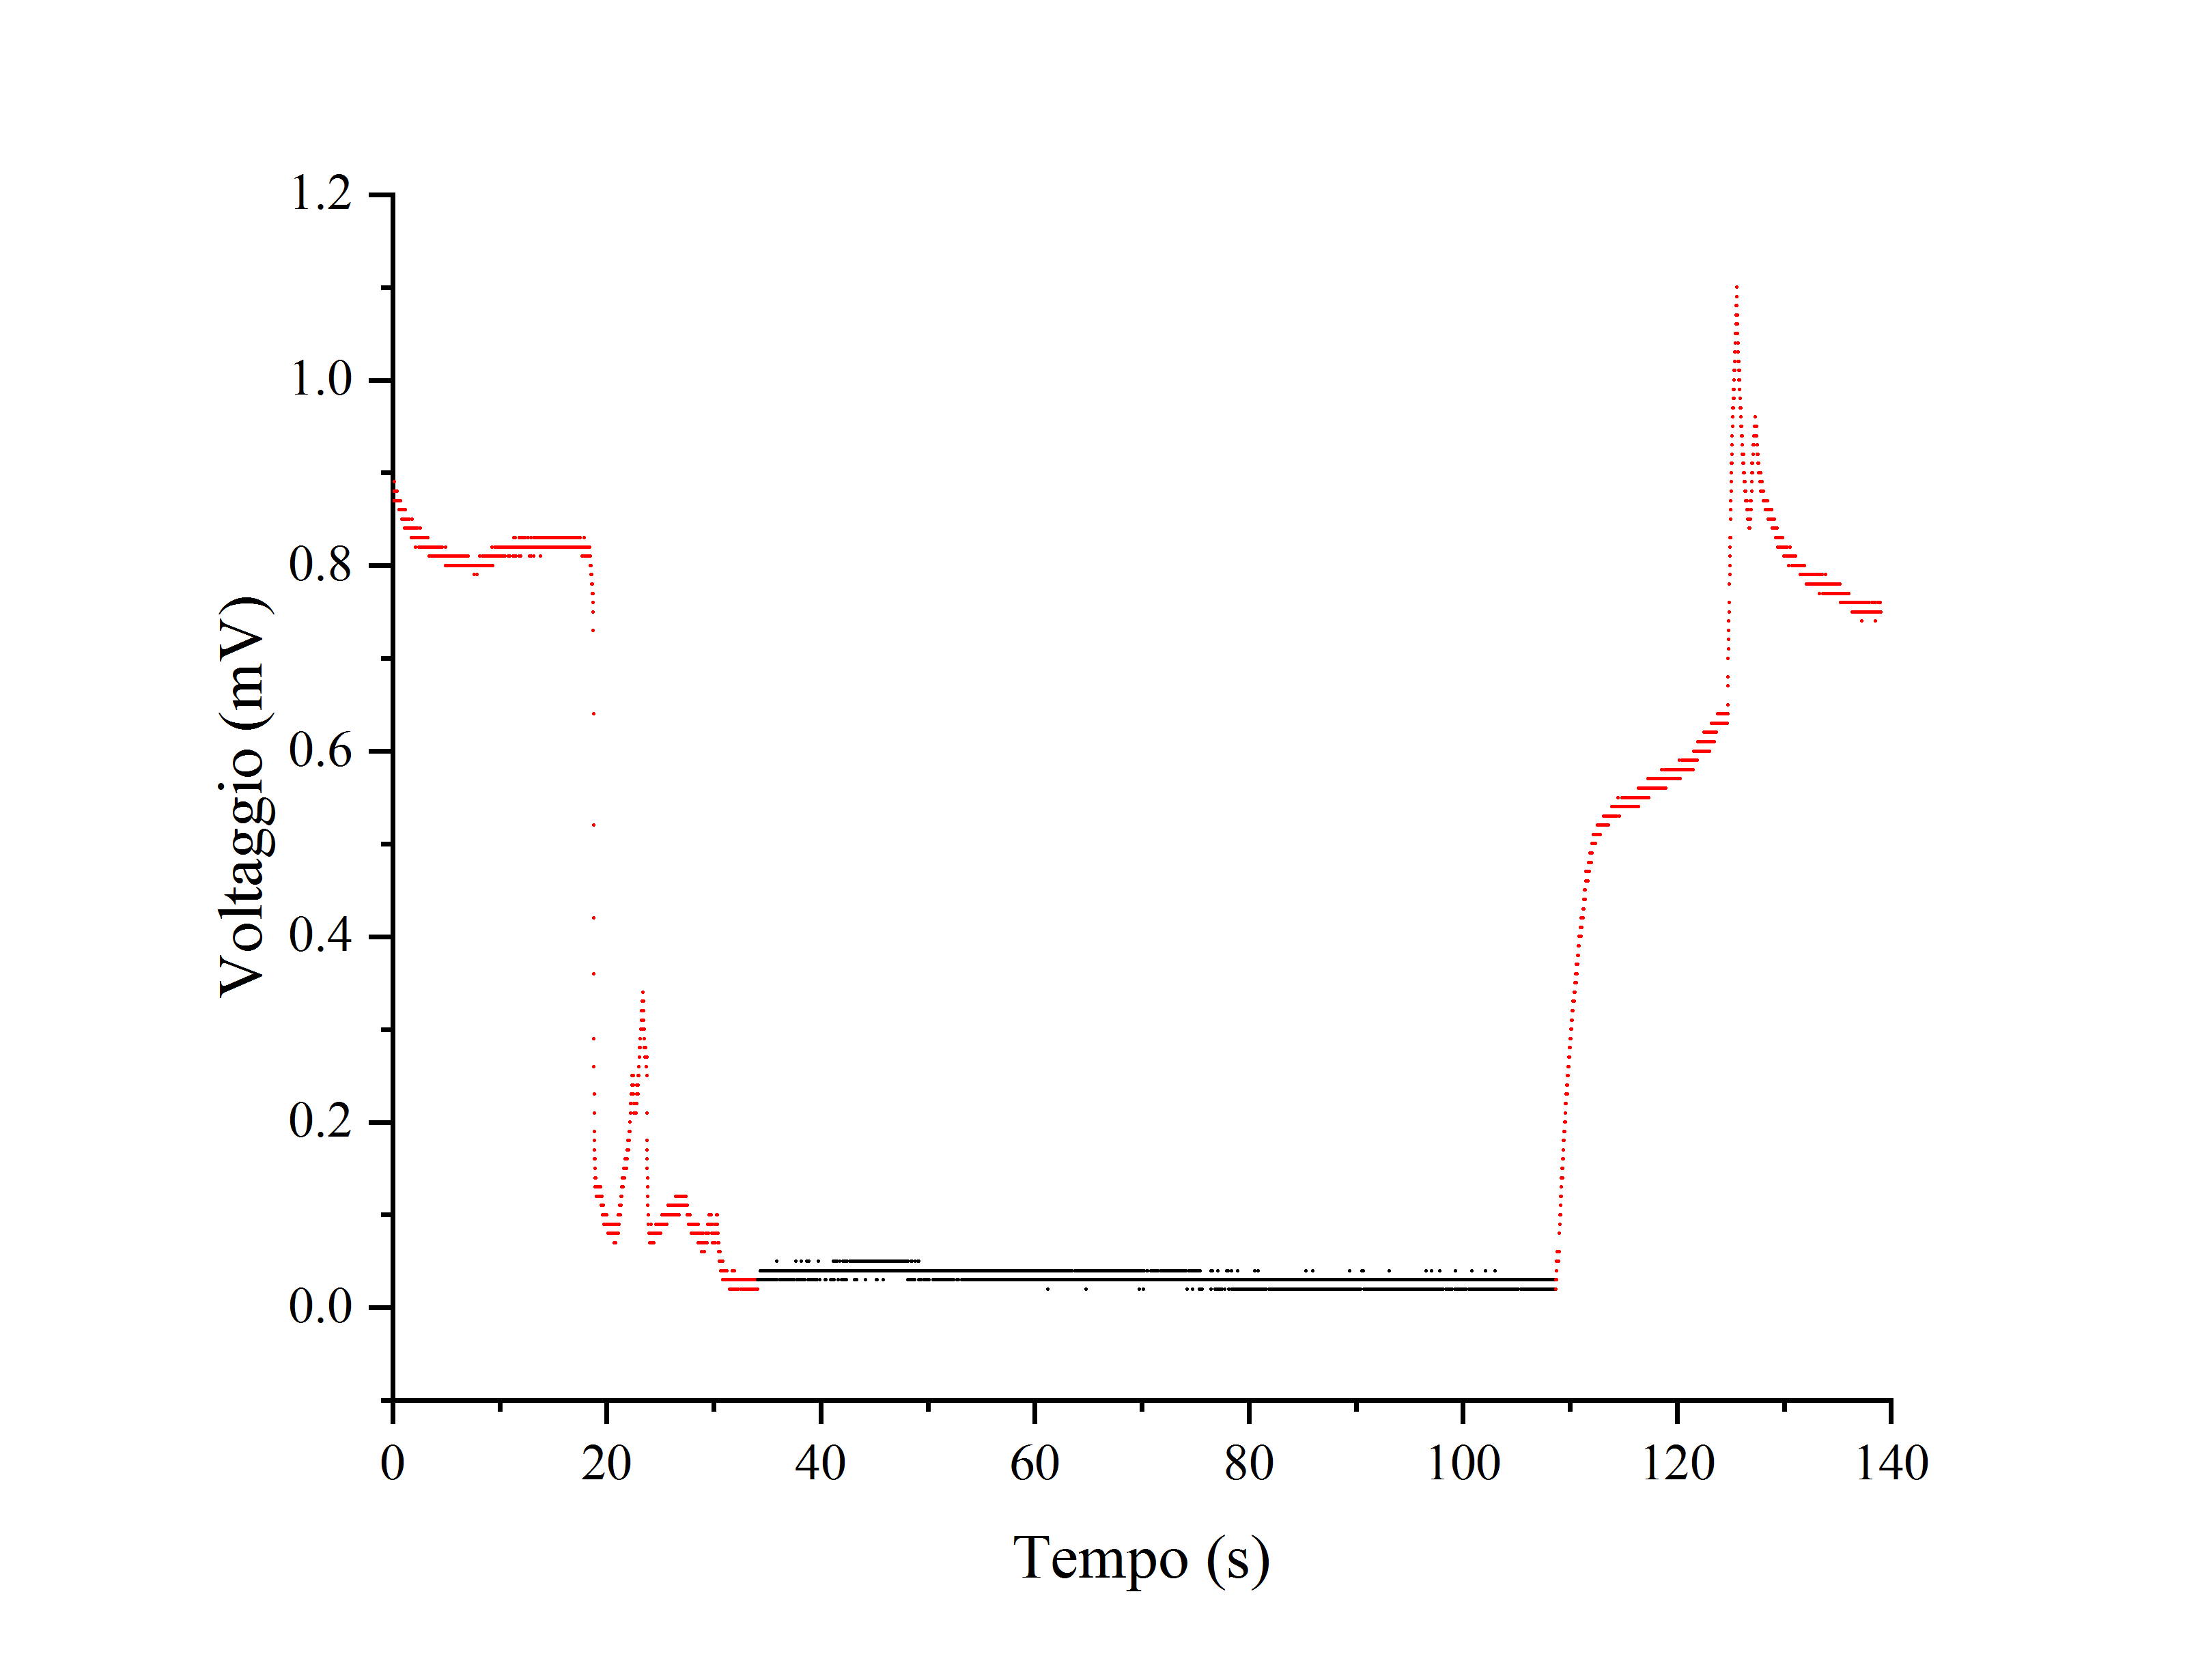
\includegraphics[trim={1cm 0.6cm 1cm 1cm},clip,width=.49\textwidth]{img/acqua-fus.png}}\hfil
  \subfloat[][
    Azoto (ebollizione)

    $\Delta V=(-5.652\pm0.013)\,\unit{mV}$
  ]{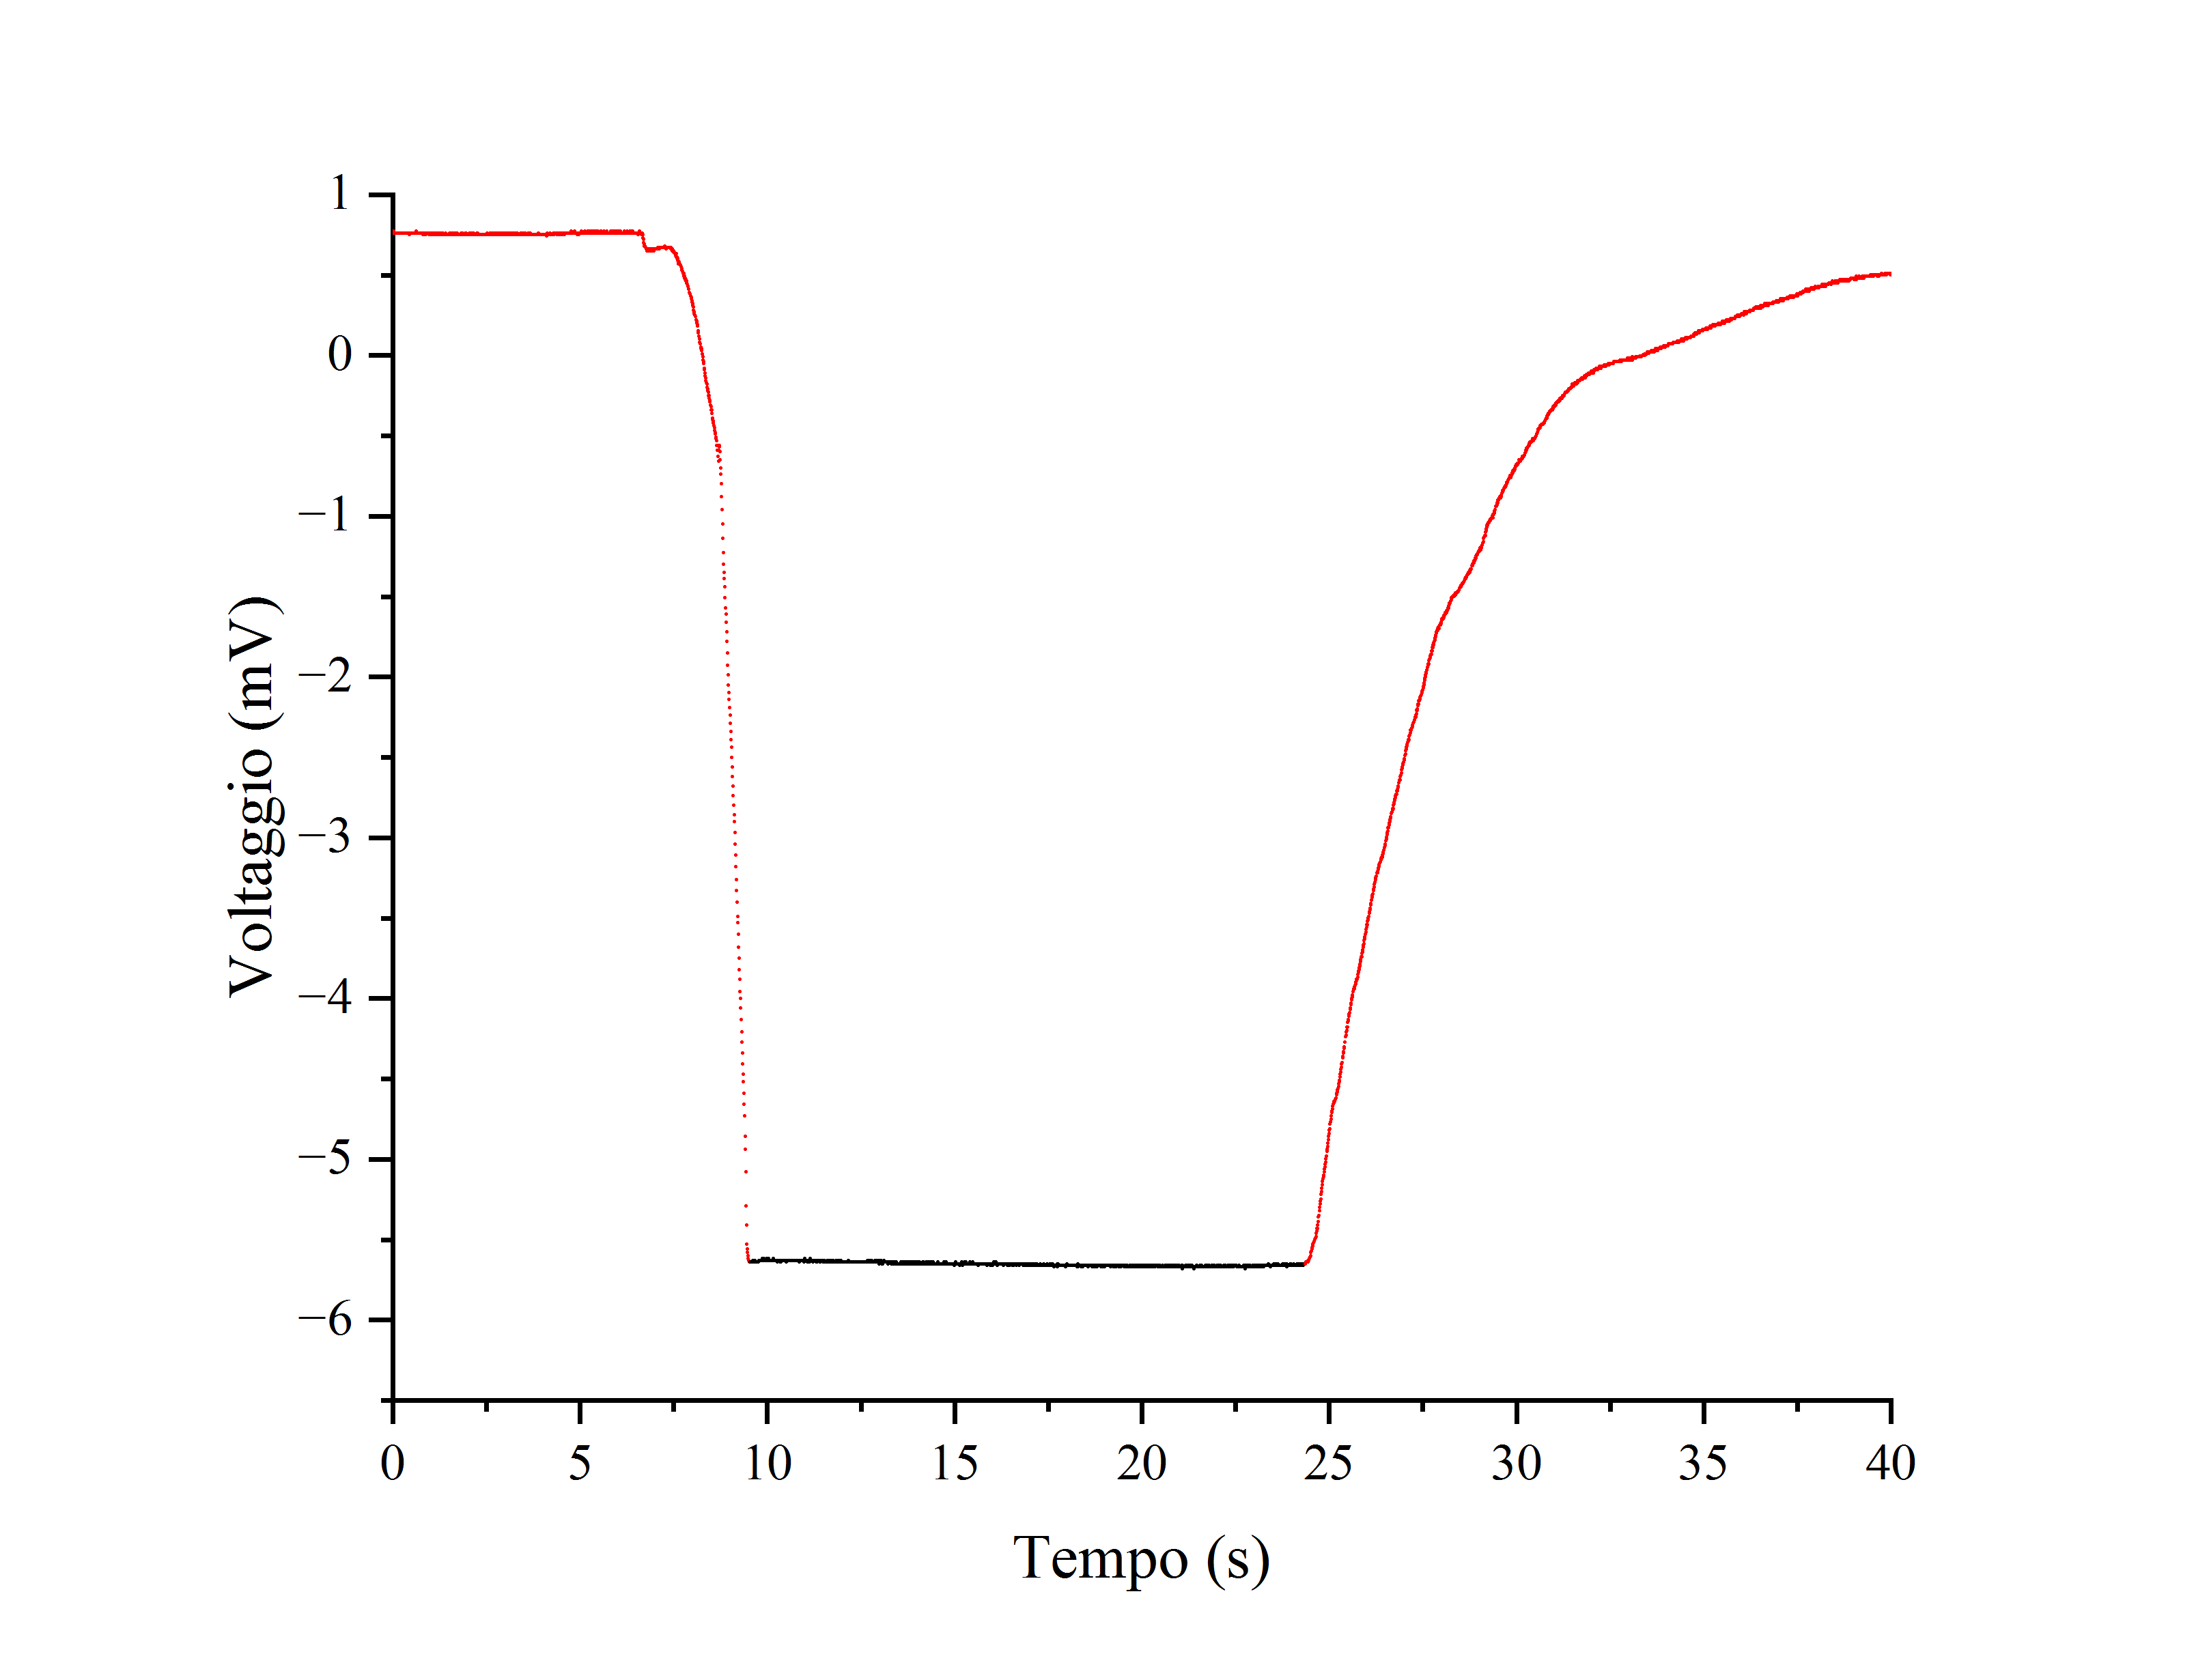
\includegraphics[trim={1cm 0.6cm 1cm 1cm},clip,width=.49\textwidth]{img/azoto.png}}\hfil
  \subfloat[][
    Acqua (ebollizione)

    $\Delta V=(3.967\pm0.010)\,\unit{mV}$
  ]{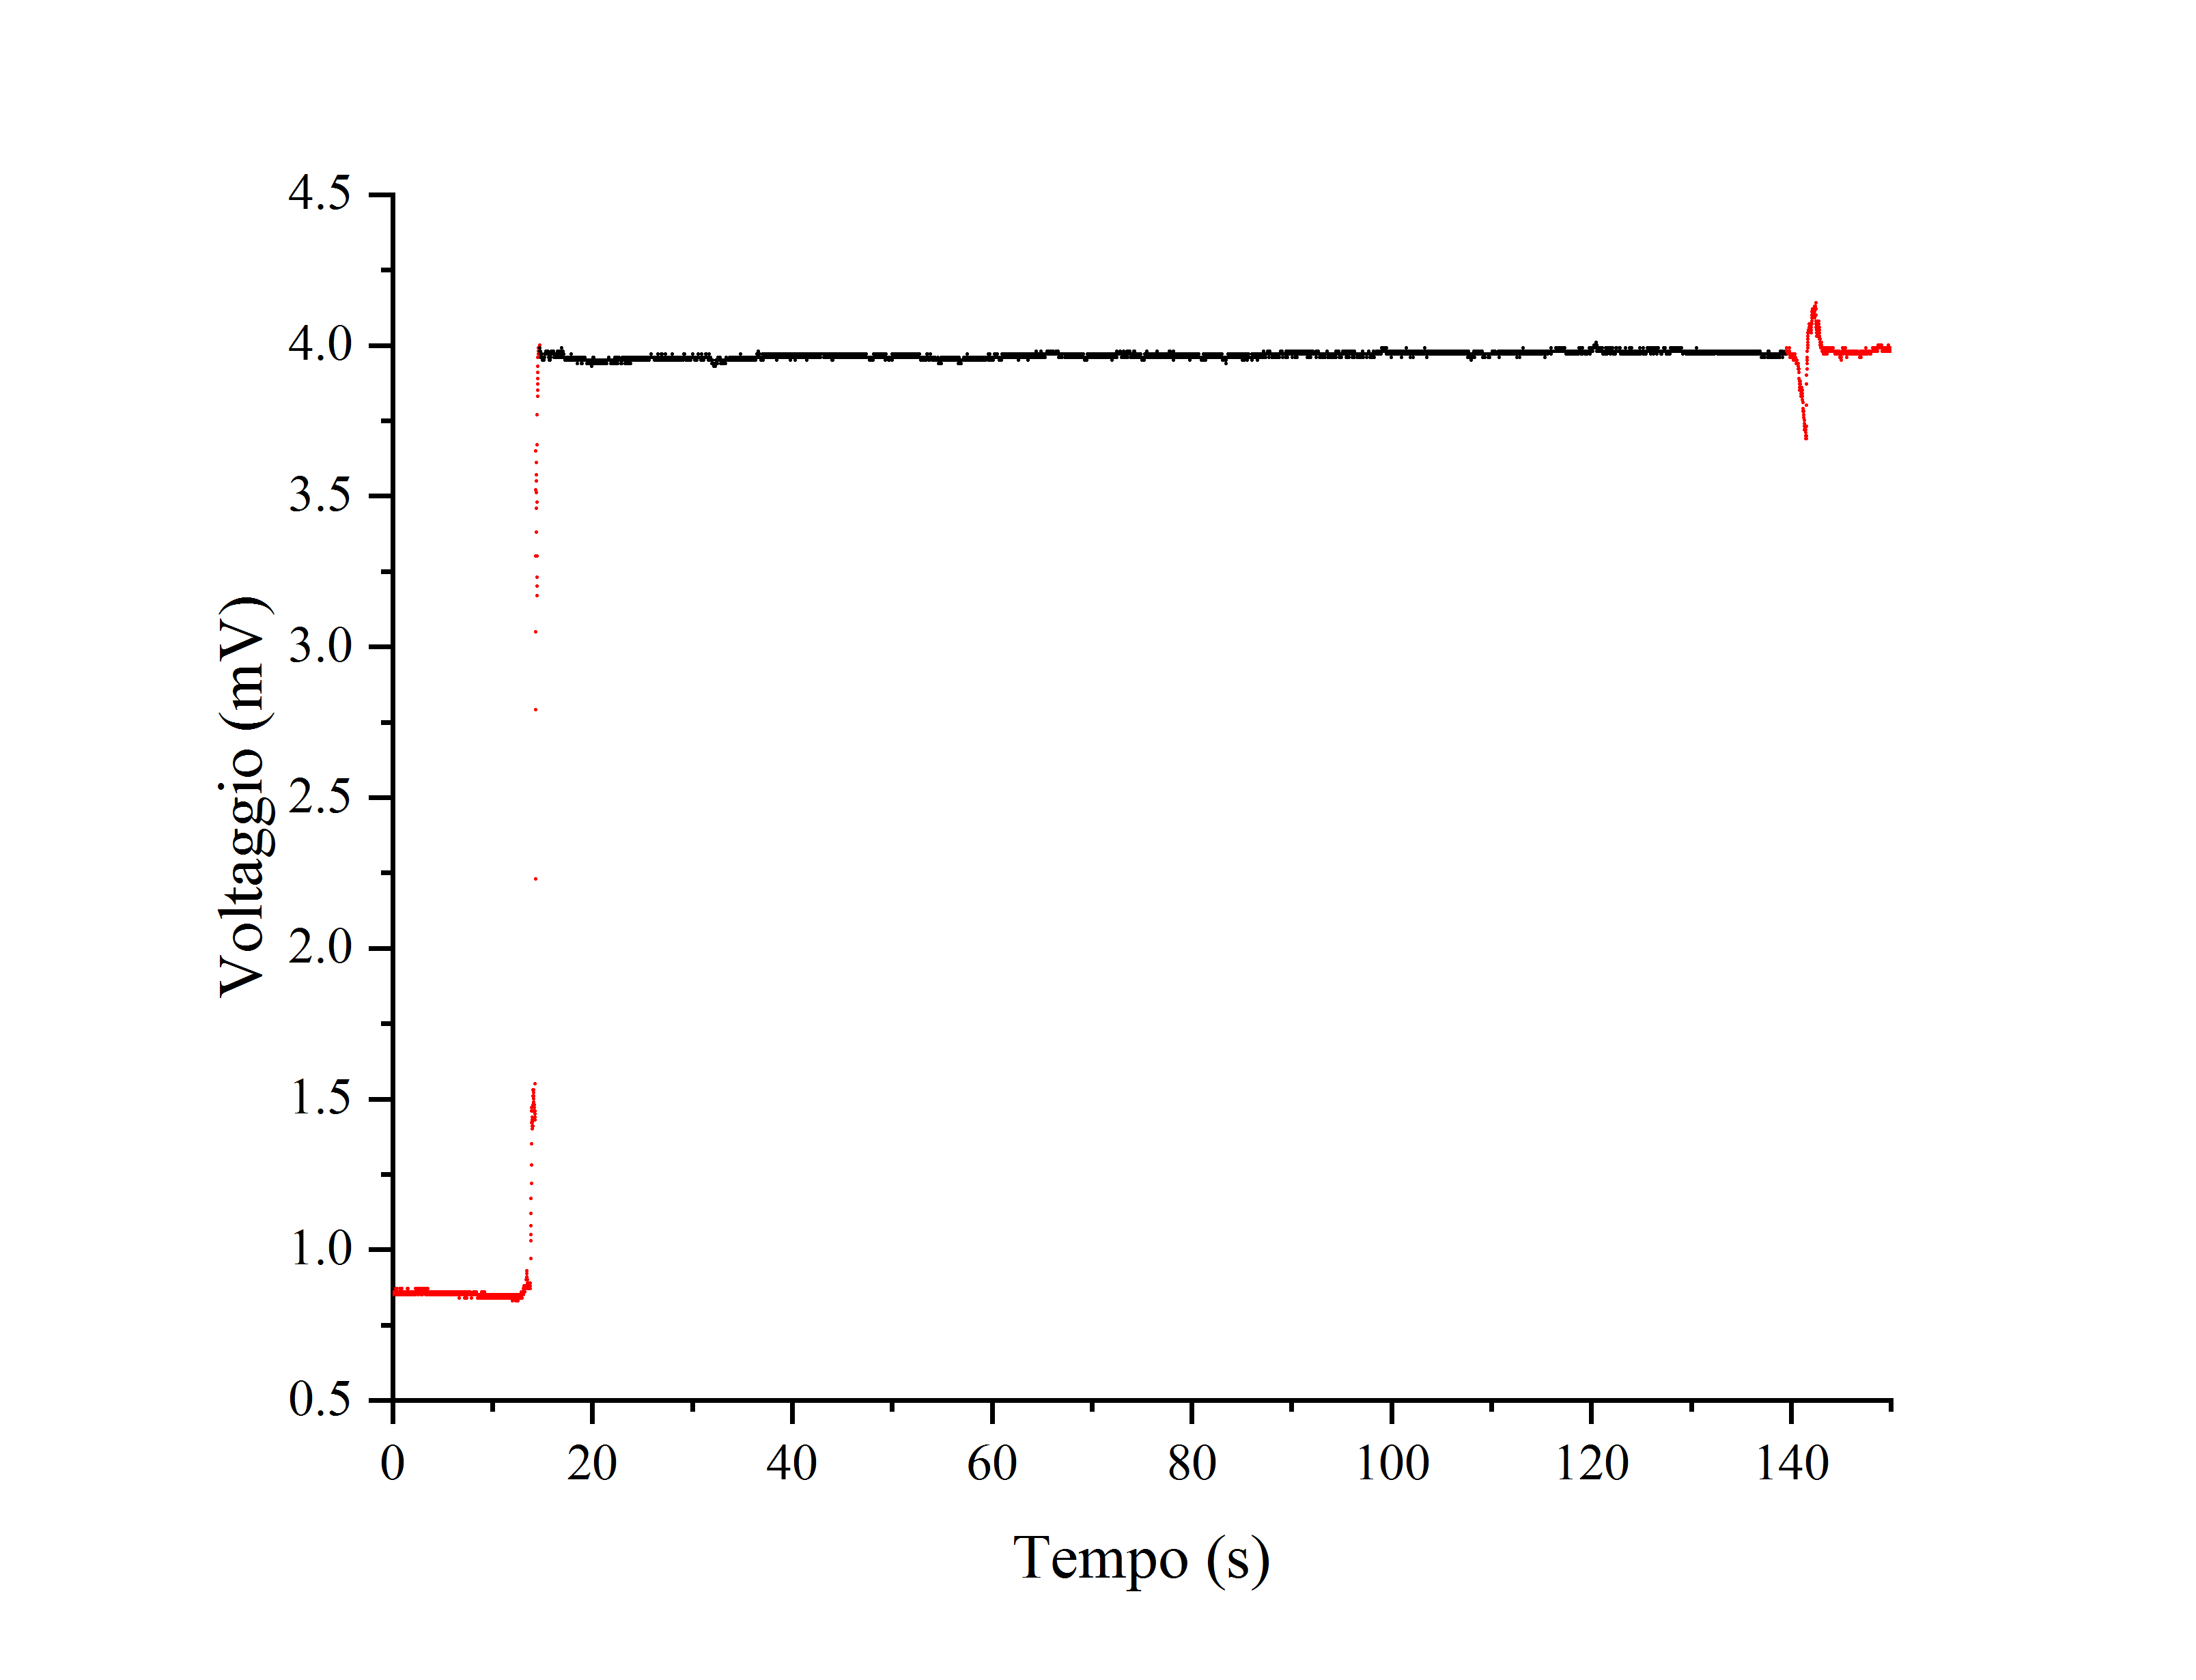
\includegraphics[trim={1cm 0.6cm 1cm 1cm},clip,width=.49\textwidth]{img/acqua-eb}}\hfil
  \subfloat[][
    Etanolo (fusione)

    $\Delta V=(-3.94\pm0.07)\,\unit{mV}$
  ]{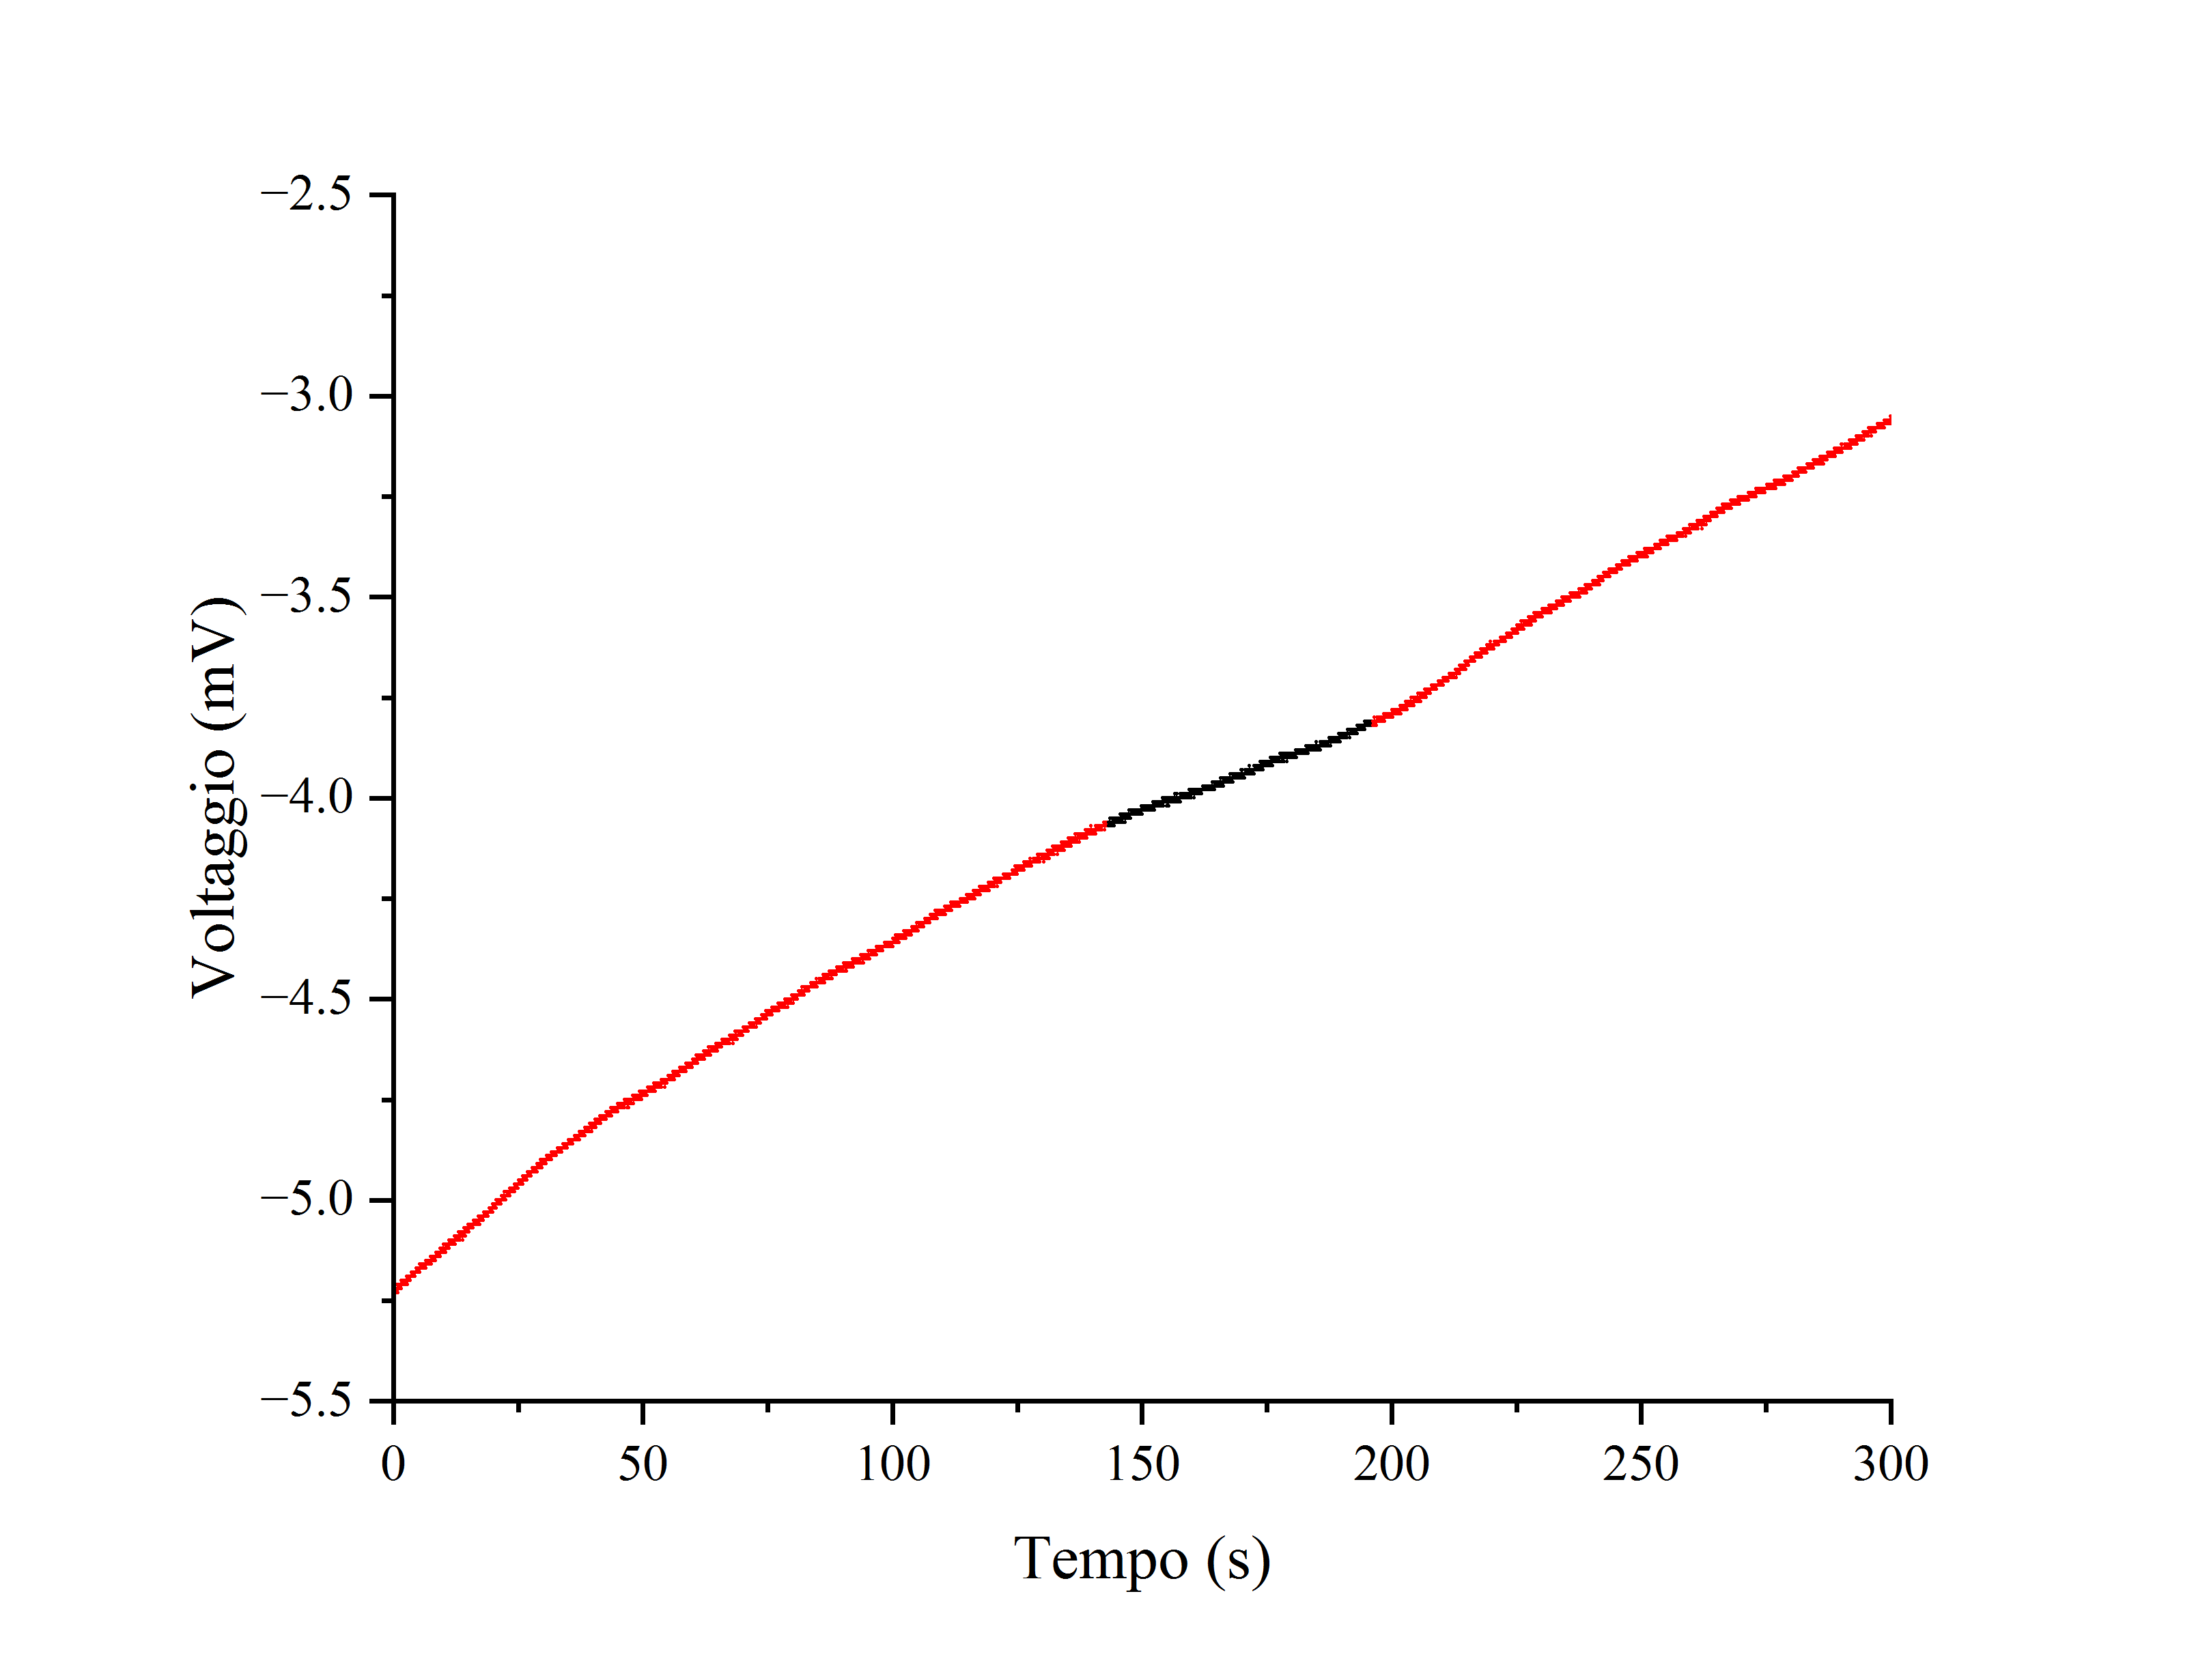
\includegraphics[trim={1cm 0.6cm 1cm 1cm},clip,width=.49\textwidth]{img/etanolo.png}}\hfil
  \subfloat[][
    Indio (fusione)

    $\Delta V=(6.214\pm0.017)\,\unit{mV}$
  ]{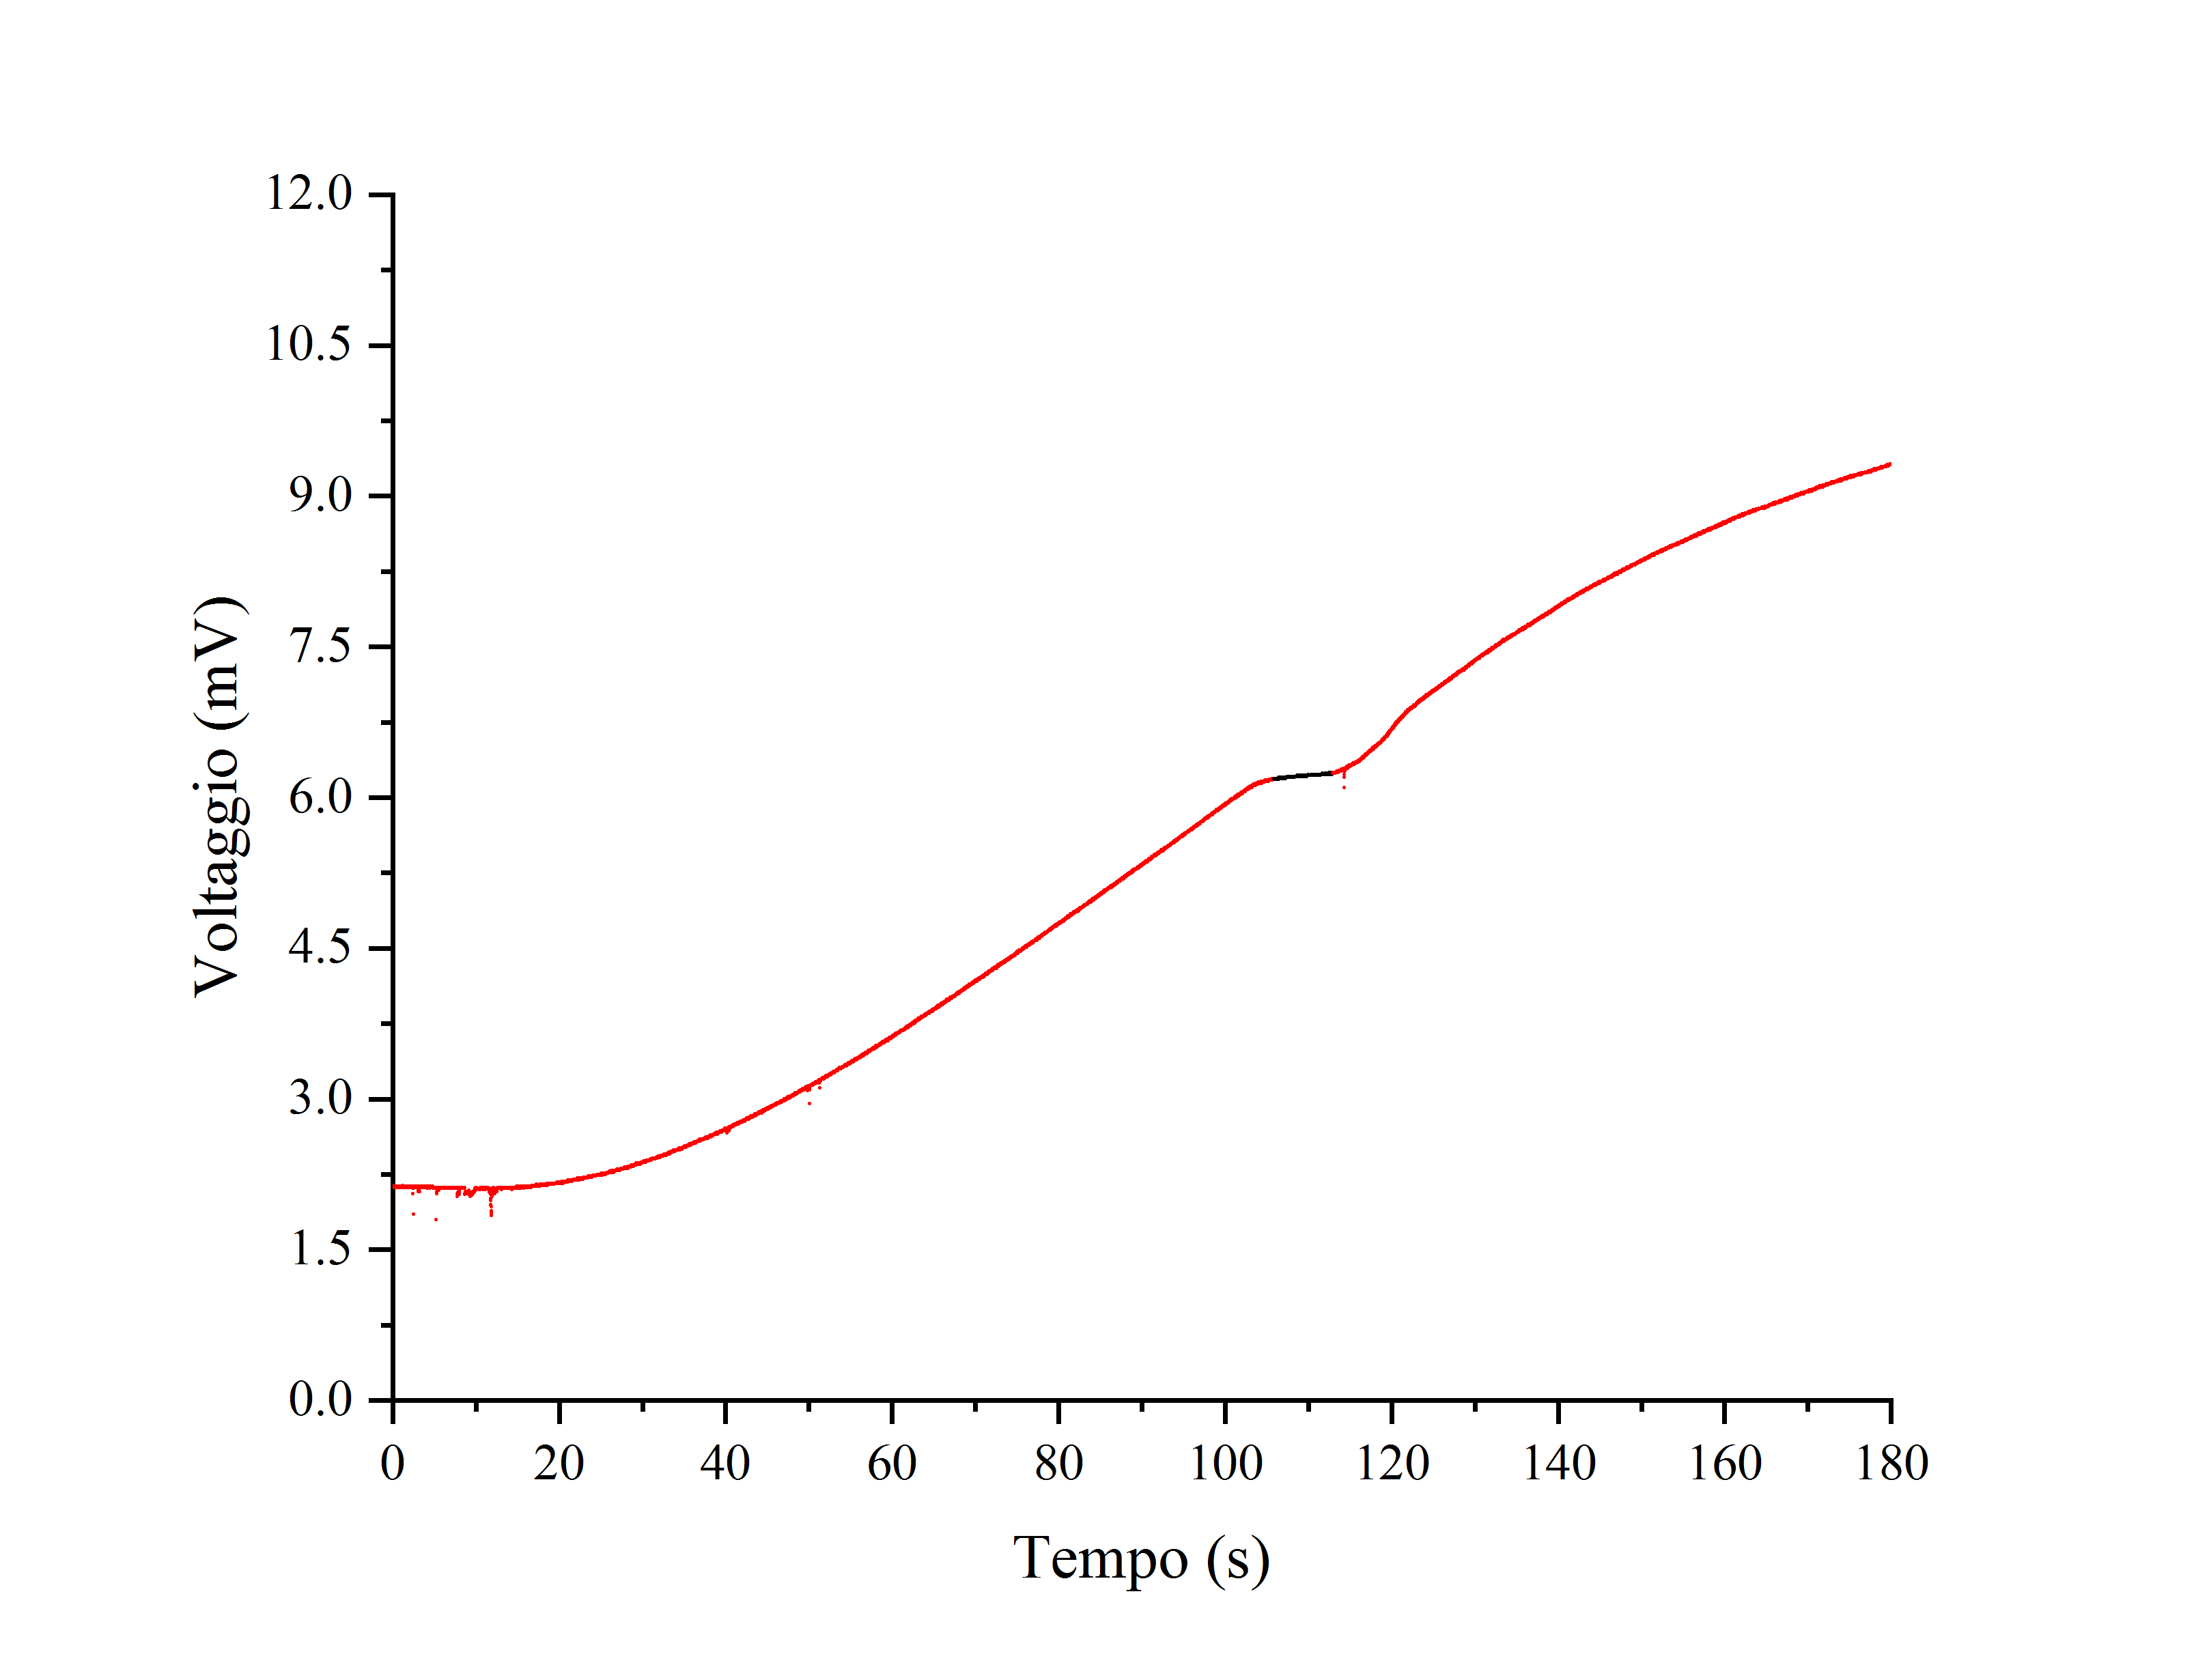
\includegraphics[trim={1cm 0.6cm 1cm 1cm},clip,width=.49\textwidth]{img/indio.png}}\hfil
  \subfloat[][
    Gallio (fusione)

    $\Delta V=(1.00\pm0.03)\,\unit{mV}$
  ]{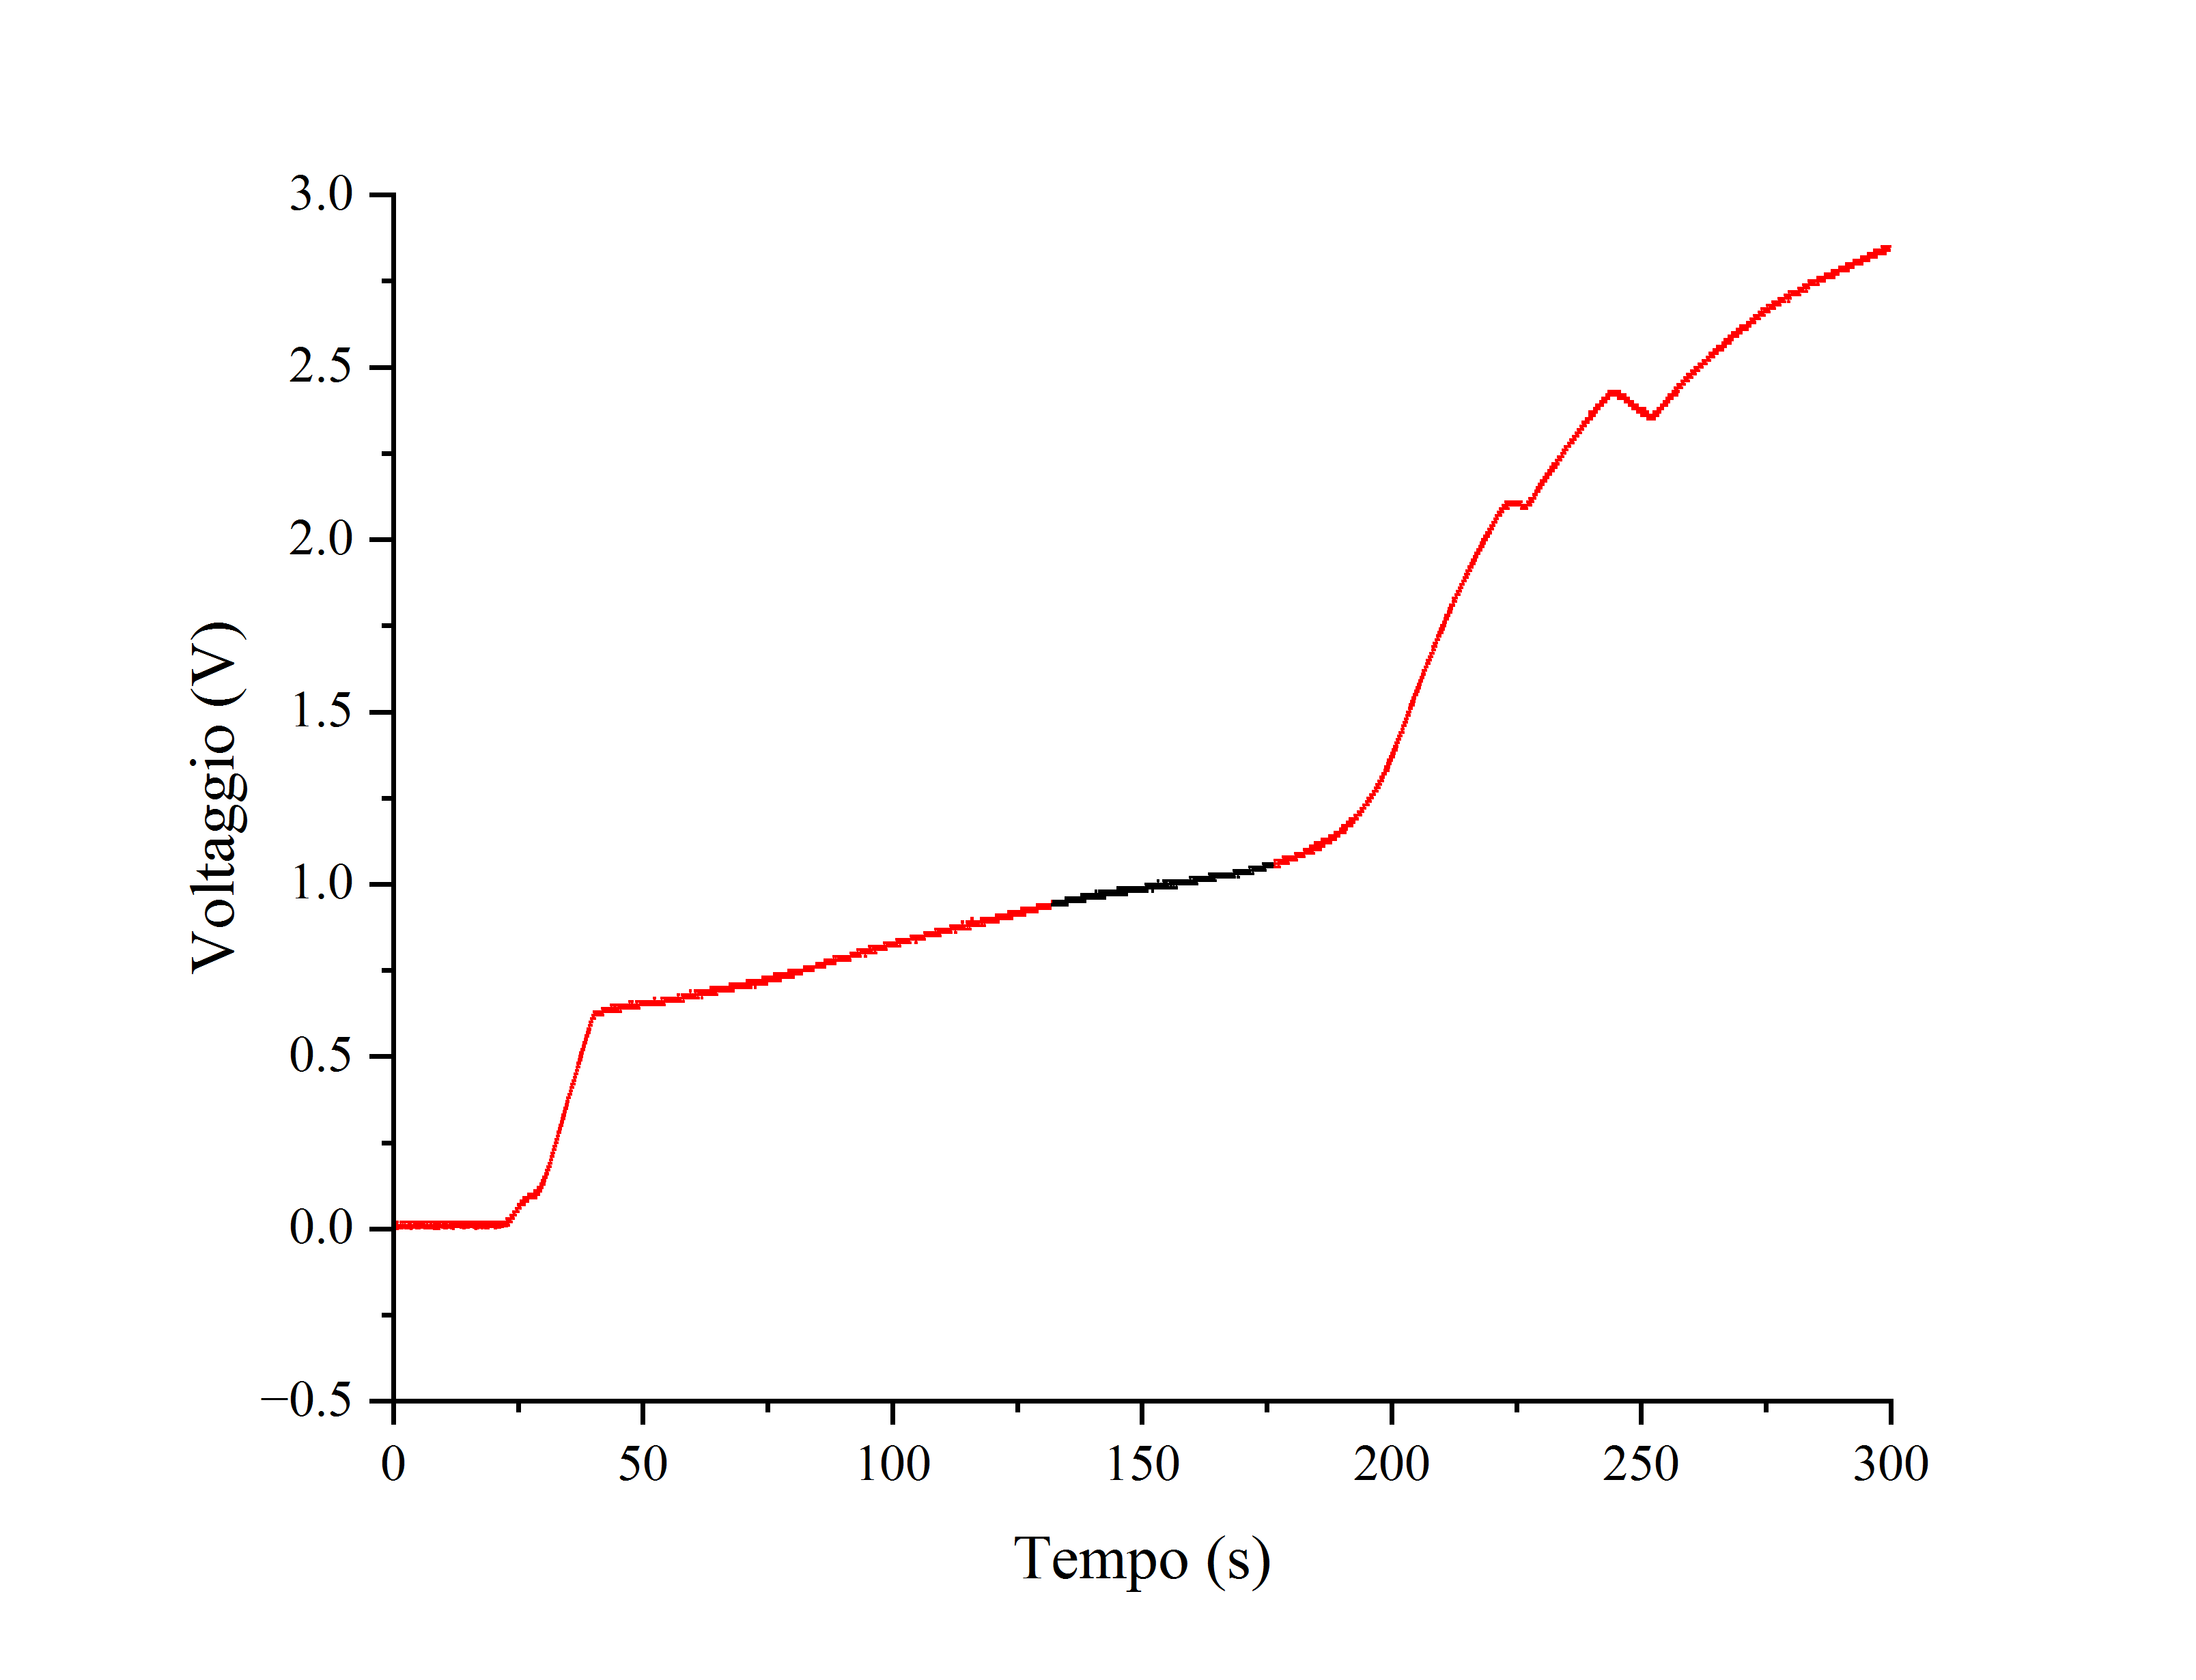
\includegraphics[trim={1cm 0.6cm 1cm 1cm},clip,width=.49\textwidth]{img/gallio.png}}
\end{figure}

\pagebreak
\subsection{Curva caratteristica della termocoppia}

Per determinare la curva di calibrazione il gruppo di lavoro ha effettuato
tre regressioni polinomiali, con polinomi di primo, secondo e terzo grado.

Abbiamo considerato come variabile indipendente la temperatura (in $\unit{K}$)
e come variabile dipendente la differenza di potenziale (in $\unit{mV}$).

\begin{figure}[H]
  \centering
  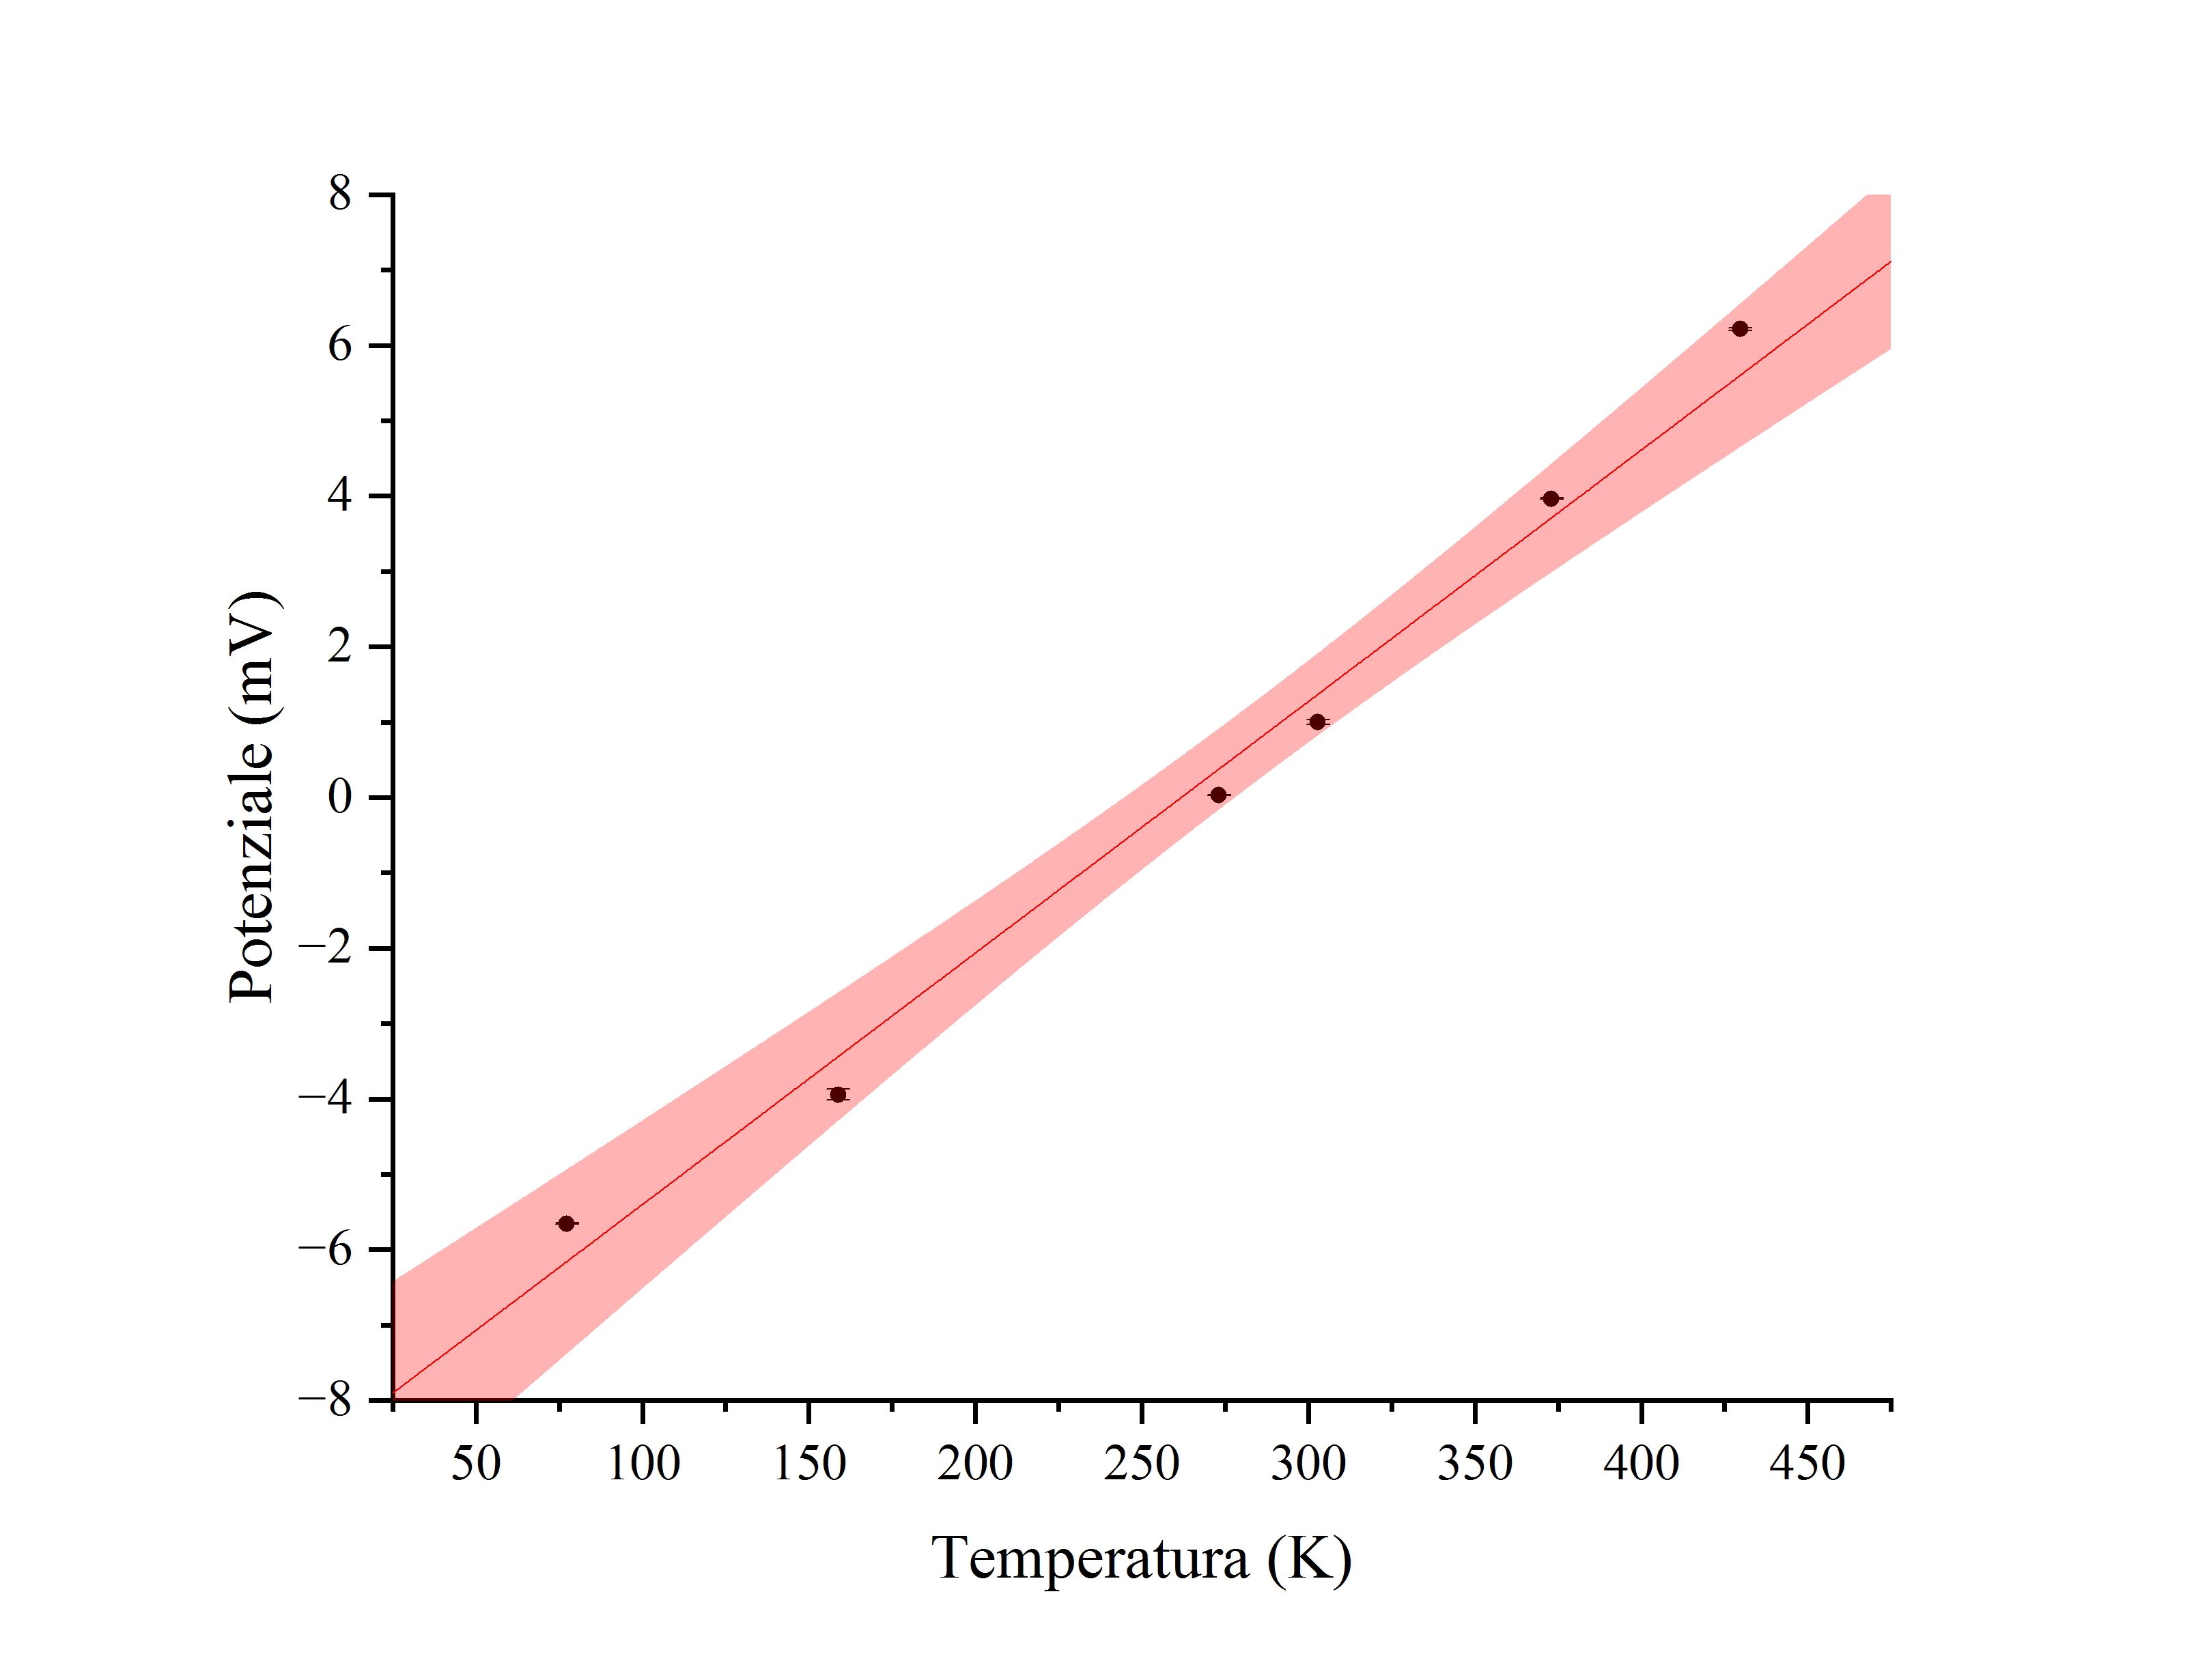
\includegraphics[trim={2cm 0.6cm 3cm 1cm},clip,width=\textwidth]{img/regressione1.png}
  \caption*{\emph{
    In rosso, la curva di regressione; in rosa, la sua regione di incertezza.
  }}
\end{figure}

Equazione della curva di regressione:
\[\begin{aligned}\Delta V_\text{lineare}(T)
  &= (3.337\pm0.005)\cdot10^{-2}\,\unit{mV\,K^{-1}}\cdot T \\
  &+ (-8.735\pm0.015)\,\unit{mV}
\end{aligned}\]

Soluzione di $
  \Delta V_\text{lineare}(T_\text{ambiente}) -
  \Delta V_\text{ambiente} = \qty{0}{mV}$:
\[T_\text{ambiente}
  = (287.29\pm1.17)\,\unit{K}
  = (14.14\pm1.17)\,\unit{\degree C}
\]

\pagebreak
\begin{figure}[H]
  \centering
  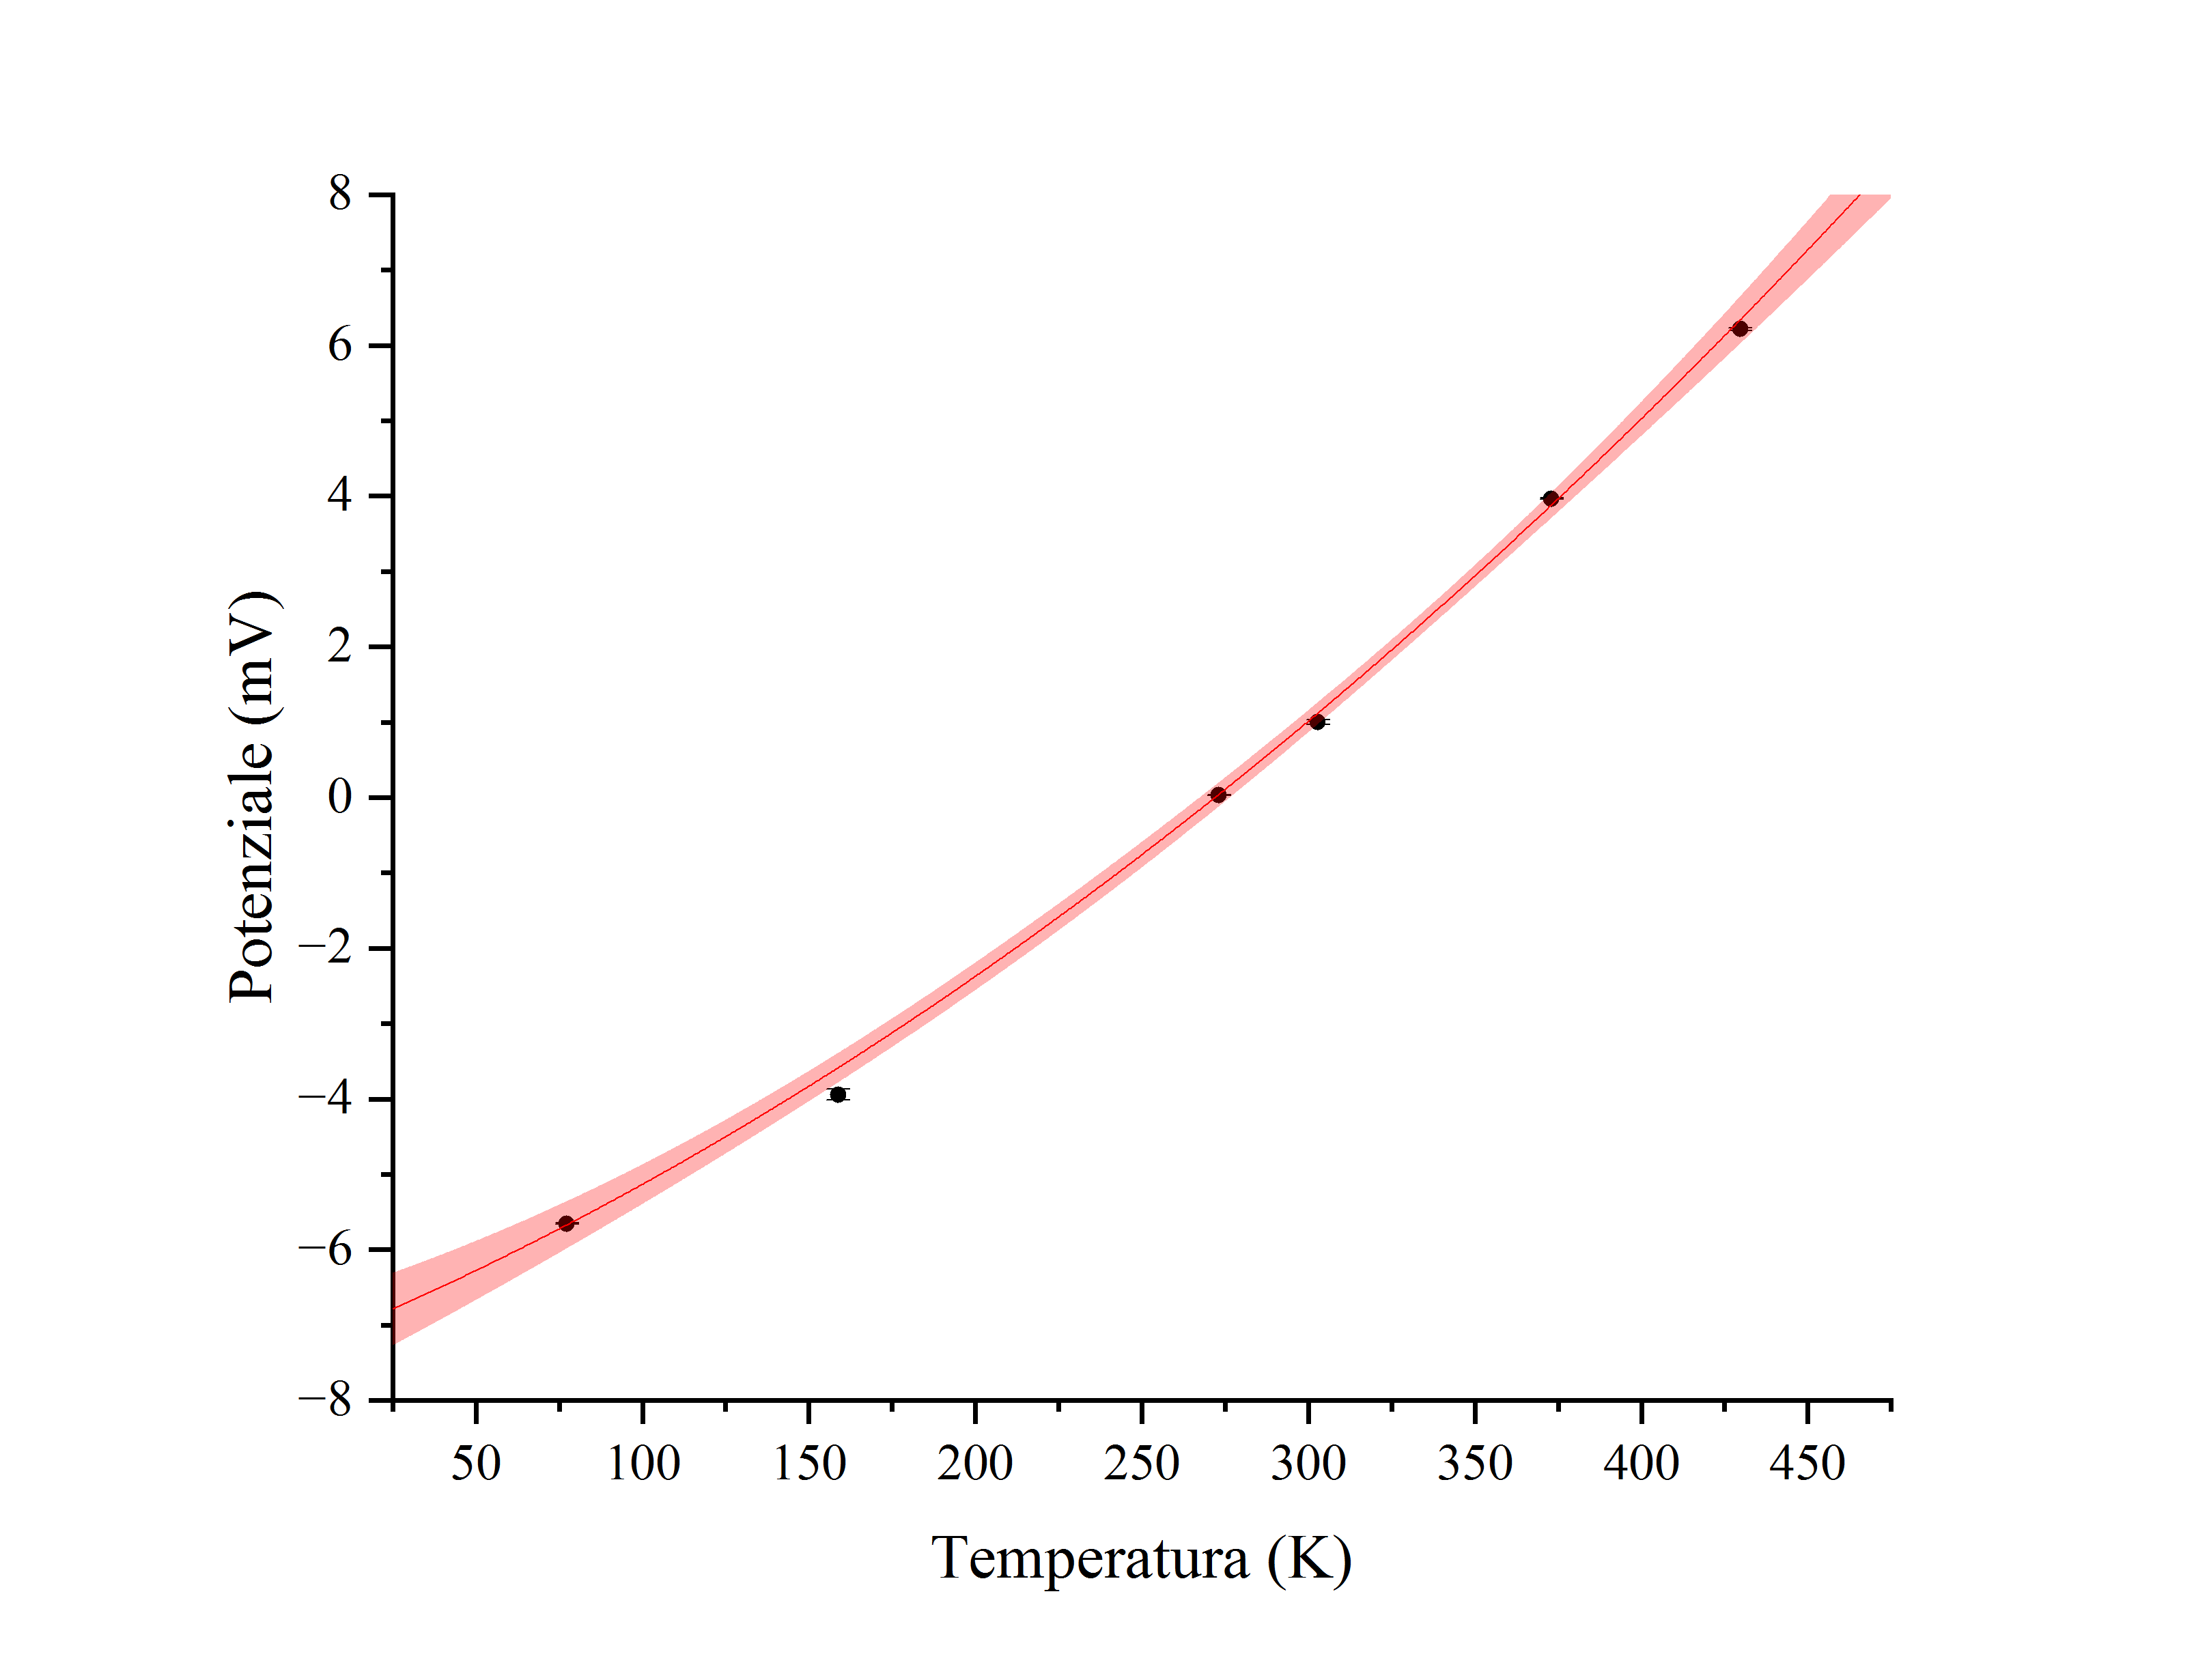
\includegraphics[trim={2cm 0.6cm 3cm 1cm},clip,width=\textwidth]{img/regressione2.png}
  \caption*{\emph{
    In rosso, la curva di regressione; in rosa, la sua regione di incertezza.
  }}
\end{figure}

Equazione della curva di regressione:
\[\begin{aligned}\Delta V_\text{quadratica}(T)
  &= (3.13\pm0.04)\cdot10^{-5}\,\unit{mV\,K^{-2}}\cdot T^2 \\
  &+ (1.82\pm0.02)\cdot10^{-2}\,\unit{mV\,K^{-1}}\cdot T \\
  &+ (-7.26\pm0.02)\,\unit{mV}
\end{aligned}\]

Soluzione (accettabile) di $
  \Delta V_\text{quadratica}(T_\text{ambiente}) -
  \Delta V_\text{ambiente} = \qty{0}{mV}$:
\[T_\text{ambiente}
  = (295.6\pm2.1)\,\unit{K}
  = (22.4\pm2.1)\,\unit{\degree C}
\]

\pagebreak
\begin{figure}[H]
  \centering
  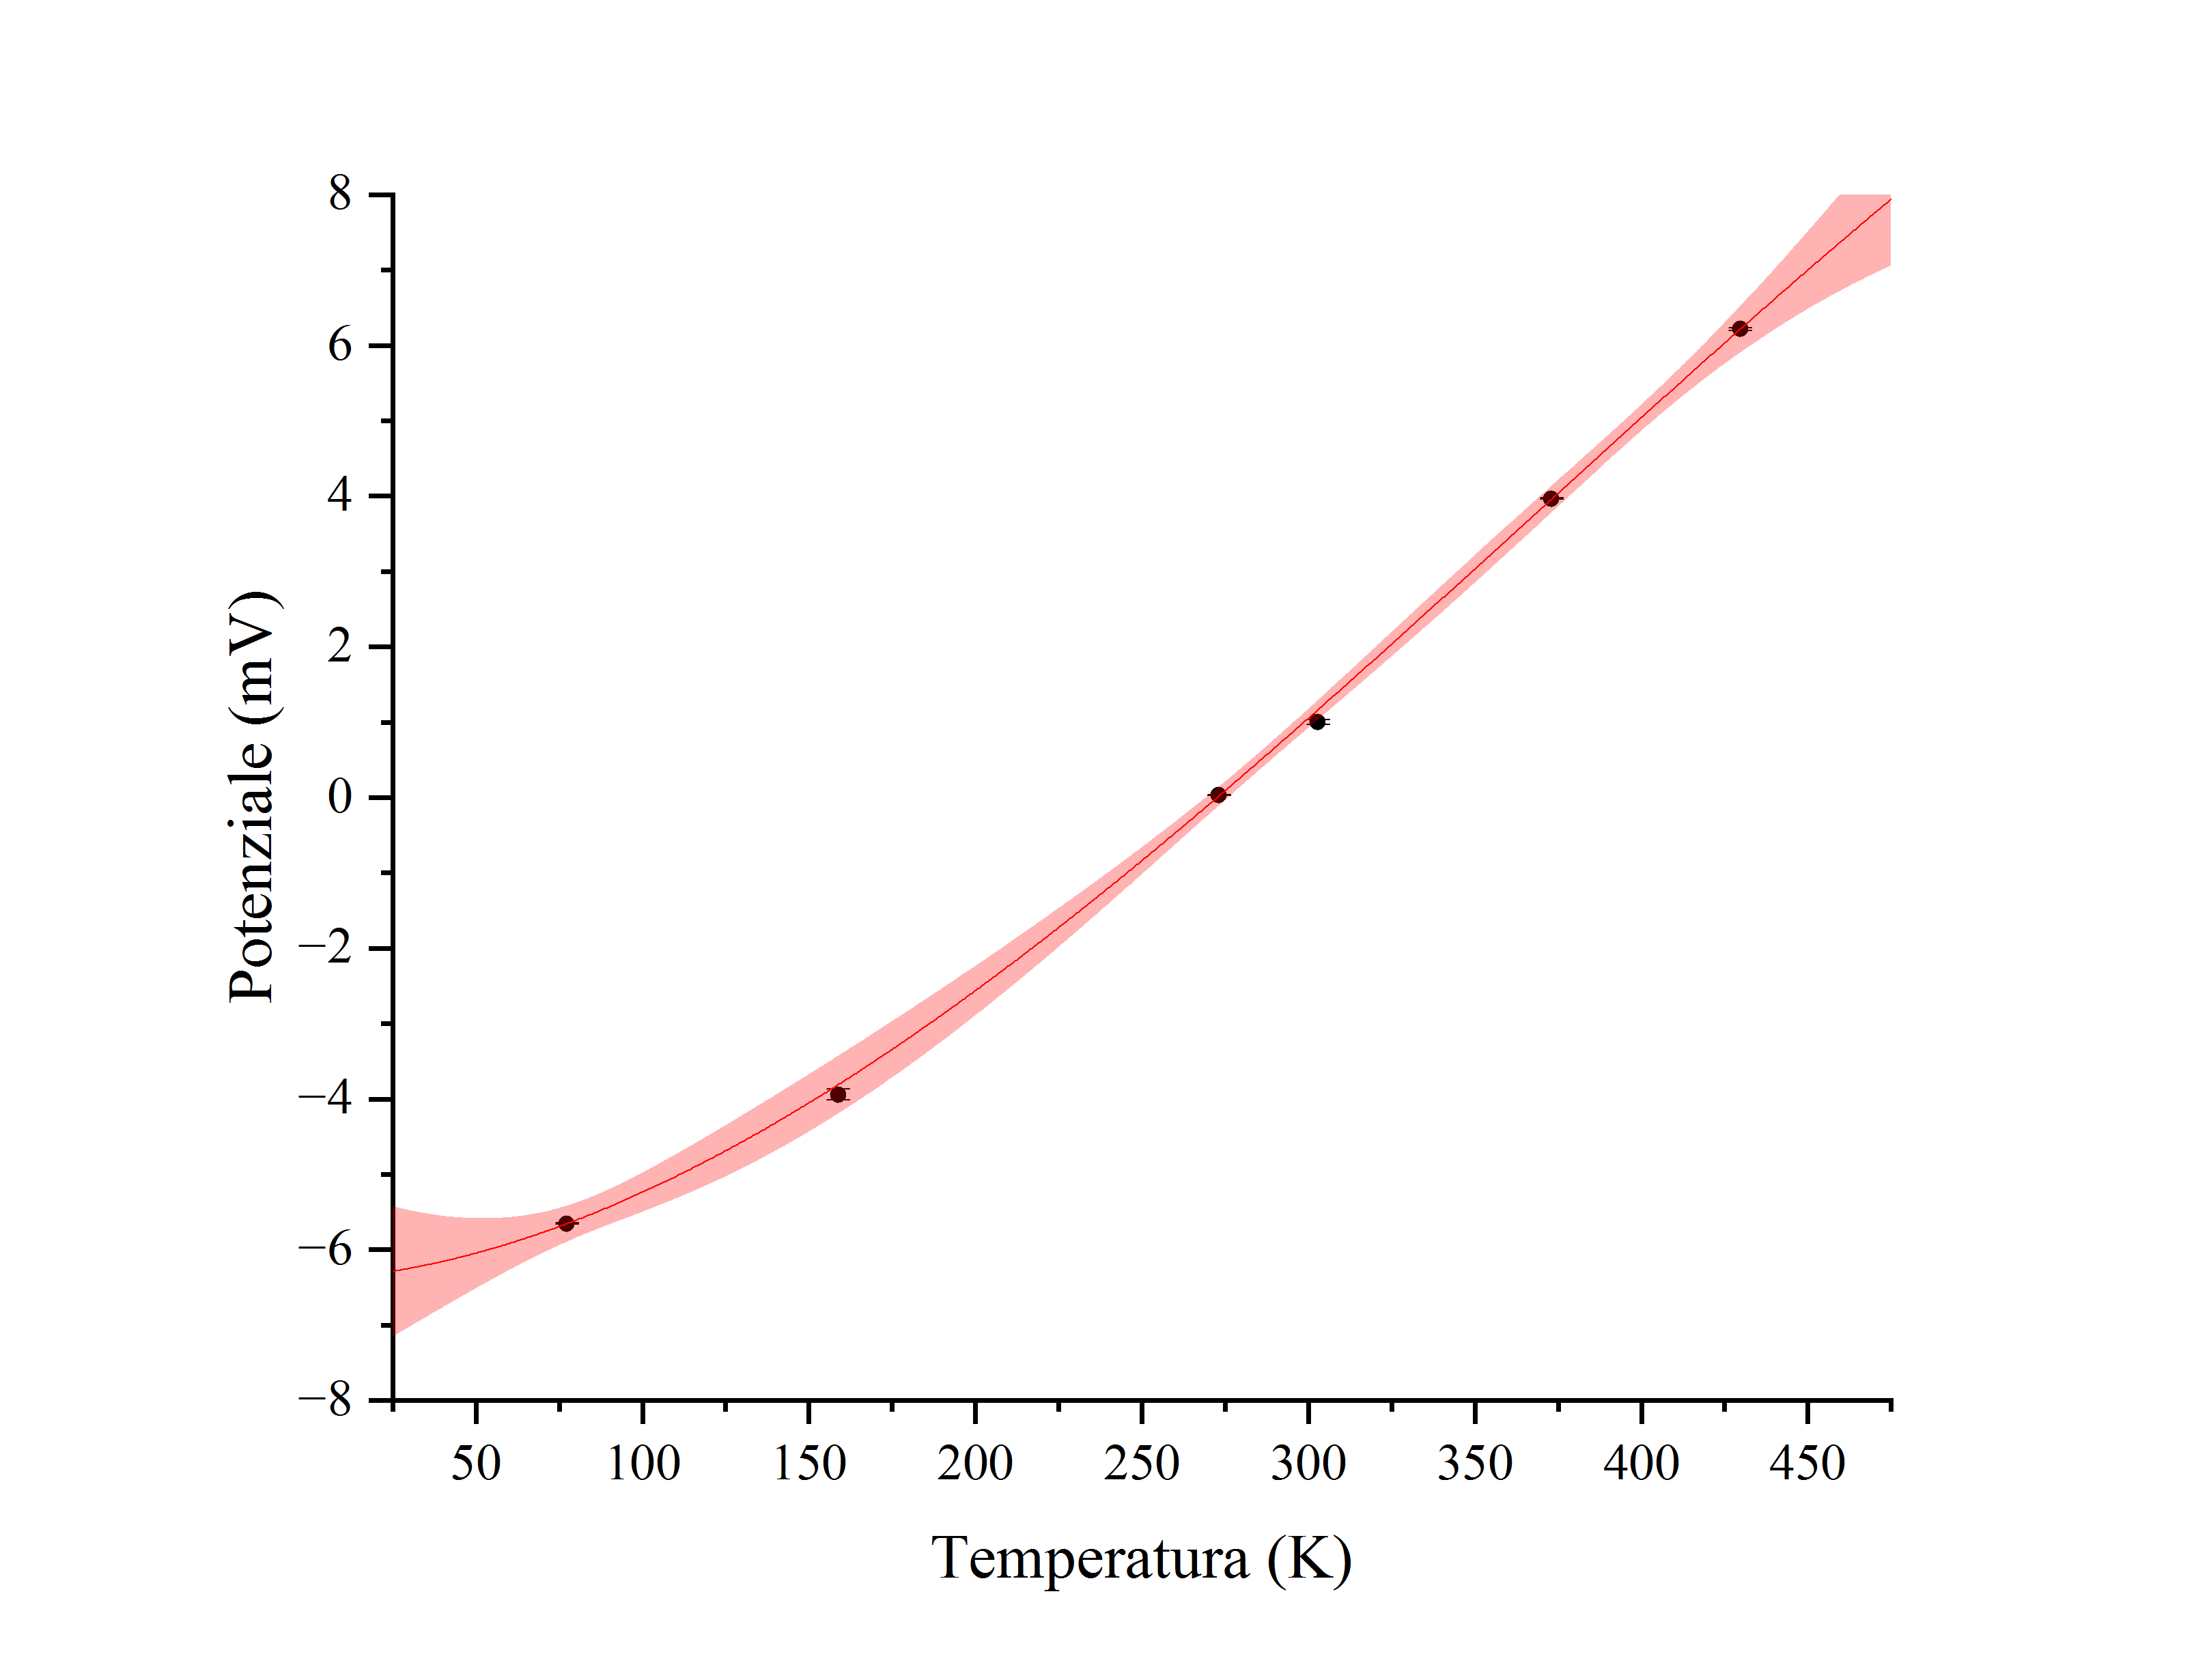
\includegraphics[trim={2cm 0.6cm 3cm 1cm},clip,width=\textwidth]{img/regressione3.png}
  \caption*{\emph{
    In rosso, la curva di regressione; in rosa, la sua regione di incertezza.
  }}
\end{figure}

Equazione della curva di regressione:
\[\begin{aligned}\Delta V_\text{cubica}(T)
  &= (-9.4\pm0.8)\cdot10^{-8}\,\unit{mV\,K^{-3}}\cdot T^3 \\
  &+ (10.3\pm0.6)\cdot10^{-5}\,\unit{mV\,K^{-2}}\cdot T^2 \\
  &+ (0.23\pm0.14)\cdot10^{-2}\,\unit{mV\,K^{-1}}\cdot T \\
  &+ (-6.41\pm0.08)\,\unit{mV}
\end{aligned}\]

Soluzione (accettabile) di $
  \Delta V_\text{cubica}(T_\text{ambiente}) -
  \Delta V_\text{ambiente} = \qty{0}{mV}$:
\[T_\text{ambiente}
  = (294.8\pm18.2)\,\unit{K}
  = (21.6\pm18.2)\,\unit{\degree C}
\]

\pagebreak
\subsection{Interpolazione della temperatura ambiente}
In alcune misurazioni di $\Delta V(t)$ abbiamo iniziato
ad acquisire dati a temperatura ambiente: questo ci ha
permesso di effettuare una valutazione dell'accuratezza
delle curve ottenute determinando $T_\text{ambiente}$
per interpolazione.

In particolare, abbiamo utilizzato
$\Delta V_\text{ambiente} = (0.85\pm0.01)\,\unit{mV}$,
media delle differenze di potenziale registrate a temperatura
ambiente.

Per valutare numericamente l'accuratezza di ogni curva
abbiamo calcolato, per ciascuna, il seguente valore (numero puro):
\[
  \varepsilon = \frac{
    \left(T_\text{ambiente,interpolata}\right)_\text{best} -
    \left(T_\text{ambiente,misurata}\right)_\text{best}
  }{\delta T_\text{ambiente,interpolata} + \delta T_\text{ambiente,misurata}}
\]
Allora $T_\text{ambiente,interpolata}$ è consistente con
$T_\text{ambiente,misurata}$ se e solo se $\left|\varepsilon\right|\le 1$;
inoltre, più $\varepsilon$ è vicino a $0$, più accurata è l'interpolazione
(e, di conseguenza, anche la stima della curva).

Per calcolare $T_\text{ambiente,interpolata}$ abbiamo determinato le radici di
\[ \Delta V(T) - \Delta V_\text{ambiente} \]

\end{document}
